\documentclass[noframe,twoside]{ncuthesisCJK}   
\usepackage{makeidx}             % for index
\usepackage{layout}
\usepackage[]{todonotes}
\dept{機械工程研究所}
\degree{碩/博士}
\title{模版 {\sf ncuthesisCJK} 使用說明}
\subtitle{\sf An example in \LaTeX/Xe\LaTeX}
%\subtitle{}=空白
\author{羅吉昌}
\mprof{羅吉昌}
\sprof{共同指導: 甲教授\\ \hspace{2.3cm} 乙教授}                         % 填入"共同指導: 某某某"
\degreedate{中~華~民~國~一百零二~年~六~月}
\copyyear{2012}
\def\XeLaTeX{Xe\LaTeX}  % Only in CJK 
\def\scalefactor{1}        % define a new command
\newcommand\insertfig[3]{
\renewcommand\scalefactor{#3}
\begin{figure}[!hbt]
\centering
\includegraphics[scale=\scalefactor]{#1}
\caption{#2}
\label{Fig:#1}
\end{figure}
}
\newtheorem{thm}{定理}[chapter]
\newtheorem{pr} {作業}[chapter]
\newtheorem{pf} {證明}[chapter]
\newtheorem{algo}{演算法}[chapter]

% what follows are for watermark, mark these out if no need
%\usepackage{background}
%\SetBgContents{
\includegraphics{NCUlogo}} % need a watermark
%\SetBgAngle{0}                                           % rotate
%\SetBgColor{black!40}                                 % color
%\SetBgScale{1.5}                                          % scale
%\SetBgHshift{100}                                        % location x=0 for center
%\SetBgVshift{230}                                        % location y=0 for center
% end of watermark codes
             % 自訂巨集多 收起來
                                 % 自訂巨集少 直接寫出

%\includeonly{chapter2}          % 單獨編譯此檔
\makeindex                       % 告訴\LaTeX要做索引
\begin{document}                 % 宣告結束   本文開始
\begin{CJK}{UTF8}{bkai}          %----------------------
\CJKhorz
\fontsize{14pt}{20pt}\selectfont % 可調間距以便閱讀%
\pagenumbering{alph}             % to cheat latex
\maketitle                       % 論文封面
\setboolean{printcopyright}{true}
\maketitle                       % 書名面
\cleardoublepage
\addtocontents{toc}{~\hfill\textbf{頁次}\par}
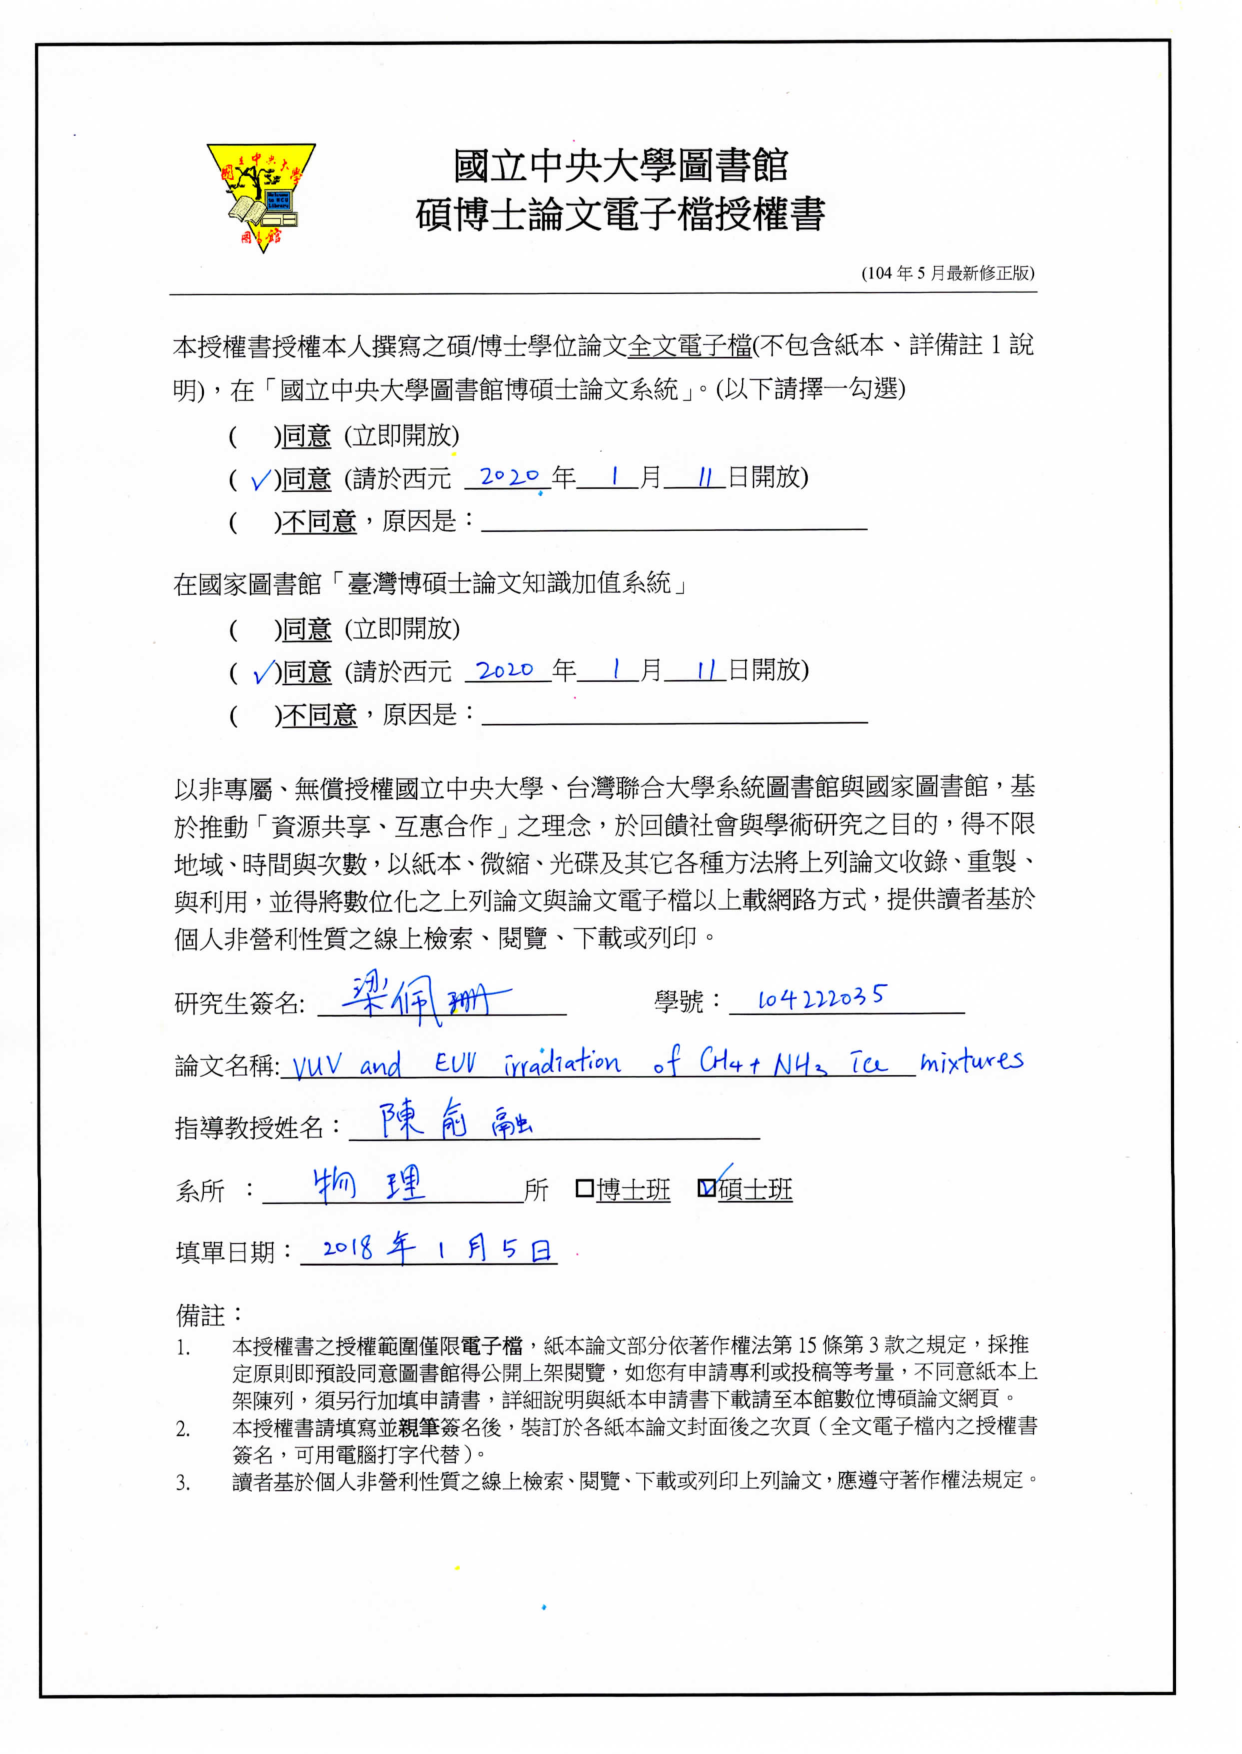
\includepdf[pages=-,scale=0.9]{myfile.pdf} % 插入其他表格
                                 % \frontmatter
\pagenumbering{roman}            % 羅馬數字編頁
\begin{abstractcn}
\index{ncuthesis 環境!abstractcn}

關鍵字:星際冰晶,冥衛一,真空紫外光,超真空紫外光
\vspace{2em}

人類從未停止對外太空的探索。為了尋找生命的起源,天文學家們觀測了一個又一個的星球。然而,除了觀測星球外,我們還能在實驗室模擬外太空的狀態,並把星際中的一些簡單份子製作出來。在實驗室模擬星際中的環境來達到探索生命起源的目的。在2002年,一群日本和美國科學家MIYAKAWA et al. (2002)\cite{miyakawa2002cold}在被稀釋的放置在-78度的環境中27年的NH$_4$CN中發現了鹼基(necleobase)的一種(adenine), 而當中CN$^-$正是胺基酸CN的來源。為了探討CN$^-$ 的生成,本文使用CH$_4$和NH$_3$在真空環境(1 $\times$ 10$^{-11}$ torr)和非常低溫(15 K)的混合物, 來模擬太陽系中的冥衛一(Charon)的表面。 我們使用真空紫外光(VUV)和超真空紫外光(EUV)來模擬太陽系中的能量來源並使用傅里葉紅外光譜儀和四極質譜儀來探討CN$^-$的生成。

\end{abstractcn} 
            % 中文摘要 abstractcn環境
\begin{abstracten}
\index{ncuthesis 環境!abstracten}

{\bf \sf Keywords:} interstellar ice, Charon, VUV irradiation, EUV irradiation

\vspace{2em}

We never stop the exploration of the outer space. Since 1900s, astronomers have observed all over the sky to seek origin of life. Apart from observing stars, we may simulate the outer space environments and make some simple molecules in laboratories on the earth now. To investigate the formation of CN$^-$, we deposite CH$_4$ and NH$_3$ (mechanism proposed by Kim and Kaiser (2011)\cite{kim}) to simulate the surface of Charon. We provide VUV and EUV irradiations as energy sources and mainly use Fourier Transform Infrared Spectrometer (FTIR) and Quadrupole Mass Spectrometer (QMS) to study different concentrations of CH$_4$ to NH$_3$ ice mixtures.

\end{abstracten} 

             % 英文摘要 abstracten
\begin{acknowledgements} \index{謝誌}
\index{ncuthesis 環境!acknowledgements}

在我的求學生涯中,有很多的老師。不過,讓我得益最多的還是這兩年多的碩士生涯。

還記得剛剛來台灣的時候,半個人都不認識,憑著老師一封電郵就來台灣唸書,實在是人生路不熟。 這兩年裡面,最感謝的人就是我的指導教授,陳俞融老師。 雖然老師對我並沒有好臉色,每次我報告完總是一副“奇怪,你怎麼又離題了”的樣子;但是我知道責之深愛之切,每次打開老師的面書,就會知道:喔,這次老師又要生我的氣了。

在整個碩士生涯中,我學會最多的就是如何篩選一篇相關的文獻,怎樣和我自己的論文相比較,從而得出究竟這篇文獻是否適用的過程。從一開始不會把整篇文獻看完,到後來認真地仔細地看別人引用的文章,再到後來自己寫出來的時候該如何引用。或者我的論文內容並不充實,但我認為碩士課程需要學習的就是如何有辨別文獻的相關性。並不是以偏概全,嘩眾取寵,而是只把自己有把握的地方讚寫出來。

本論文得以完成,實在是一件非常不容易的事情。由於本人英文寫作不佳,所以感謝好友Jess幫忙修改英文句子。謝謝學長samuel教我使用Latex,謝謝實驗室的學長豆花教導我做實驗,學弟妹謝妮恩,蘇映全,在同步輻射期間的幫忙。最後,還要感謝angela和gerilermo教授的寶貴意見,令我獲益良多。

\end{acknowledgements} 
            % 謝誌     acknowledge
\cleardoublepage
\phantomsection\addcontentsline{toc}{chapter}{目錄}
\tableofcontents                 % toc
\cleardoublepage
\phantomsection\addcontentsline{toc}{chapter}{圖目錄}
\renewcommand{\numberline}[1]{圖~#1\hspace*{1em}}%圖目錄
\listoffigures                   % lof
\cleardoublepage
\renewcommand{\numberline}[1]{表~#1\hspace*{1em}}%表目錄
\phantomsection\addcontentsline{toc}{chapter}{表目錄}
\listoftables                    % lot
\index{\LaTeX!\textbackslash phantomsection}
\index{\LaTeX!\textbackslash addcontentline}
\index{\LaTeX!\textbackslash hspace}

\listoftodos
\todo[inline]{完稿時要用[disable]除去所有todos。}
\begin{symbols}
\index{ncuthesis 環境!symbols}
\begin{tabular}{l@{ : }l}
\textbackslash dept & {研究所}           \\[1ex]                         
\textbackslash degree & {碩/博士 or 專題研究 or 論文計畫書}     \\[1ex]                                      
\textbackslash title & {論文中文題目}  \\[1ex]
\textbackslash subtitle & {論文英文題目}  \\[1ex] 
\textbackslash logo & 封面校徽(預設中央校徽)\\[1ex]
\textbackslash author& 作者             \\[1ex]                                   
\textbackslash mprof&  指導教授          \\[1ex]                  
\textbackslash sprofi, \textbackslash sprofii& 兩位共同指導 \\[1ex]
\textbackslash degreedate& 中~華~民~國~XXX~年~X~月 \\[1ex]
\textbackslash copyyear& 著作完成年  \\[1ex]
\textbackslash includepdf & 插頁指令,需pdfpages巨集 \\[1ex]
\textbackslash fontsize\ldots\textbackslash selectfont & 設定字大小行距\\[1ex]
\textbackslash bookbone & 書脊短時用\\[1ex]
abstractcn & 中文摘要環境名,檔案則為abstractcn.tex\\[1ex]
abstracten &  中文摘要環境名,檔案則為abstracten.tex\\[1ex]
acknowledge{\color{red}ments} &  謝誌環境名,檔案則為acknowledge.tex\\[1ex]
append{\color {red}A} &  附錄一環境名,檔案則為appendix.tex\\[1ex]
append{\color {red}B} &  附錄二環境名,檔案則為appendix.tex\\[1ex]
symbol{\color {red}s} &  符號說明環境名,檔案則為symbol.tex\\[1ex]
\end{tabular}
\label{symb}
\end{symbols}                 % 符號說明     symbols 環境
\cleardoublepage

\pagenumbering{arabic}           % 阿拉伯數字編頁
                                 % \mainmatter
%\chapter{\protect Introduction}
\label{introduction}

According to Hindu cosmological mythology, ancient people believe that a giant turtle bears the world on its back. Even after we stepped onto the moon at 1969, there are still plenty that we cannot explain. Recently, a group of scientists put a dilute NH$_4$CN in temperature of liquid nitrogen for 27 years and discovered a wide variaty of pyrimidine and purines \cite{miyakawa2002cold}. NH$_4^+$CN$^-$ plays an important role in life evolution. The formation of CN$^-$ is proposed by Kim and Kaiser (2001) \cite{kim},which is produced by ammonia (NH$_3$) and methane (CH$_4$). However, they have only demonstrated the effects of energetic electrons onto the ice mixtures, the photolysis experiments of CH$_4$+NH$_3$ ice mixtures especially variating relative proportions of CH$_4$ to NH$_3$ by VUV or EUV photons has not been performed. This thesis aims to investigate the chemistry of VUV and EUV irradiations on CH$_4$+NH$_3$ ice mixtures, which is possibly one of the main starting components to form CN$^-$ in astrophysical environments.\\

NH$_3$ is often not probed in astrophysical environments unless detecting ambiguously because nearly all the infrared bands overlap with water. The "unbrella" mode (1070 cm$^{-1}$) is often obscured by the 10 micron silicate feature \cite{d1986time}. It is often detected as ammonia hydrates (NH3 $\cdot$ nH$_2$O)\cite{cook2007near}. The New Horizons team has revealed a high concentration crater of NH$_3$ on Charon\cite{grundy2016surface}. Figure \ref{fig:Charon_IR} presents the infrared spectra detected by LEISA camera regarding four different segments at the right panel. On Organa crater, we may observe a 2.2 $\mu$m absorption representing presence of ammonia at "b" spectrum. The part b spectrum is enlarged at left bottom panel with the green pigments indicates the concentration of ammonia overlapped on topological graph of Charon. This also explains the different concentration of ammonia detected by different earth-based observation groups cook et al (2007)\cite{cook2007near} and brown et al. (2000)\cite{brown2000evidence}.\\

Charon, as a member in the Pluto system, is the second massive member with masses about half of Pluto. It orbits around Pluto, where Pluto is orbiting the Sun with an semi-major axis of 39.1 A.U. and period of 248 earth years. Similar to the earth and moon system, they orbits synchronized to each other with tidal-lockings, which the same side always facing each other. The main ejecta from Pluto (5-6 $\times$ 10$^{25}$ s$^{-1}$ from the New Horizons observation) is CH$_4$ (99\%), with net depositional flux of 4 $\times$ 10$^{24}$ s$^{-1}$ (98 \% of which are CH$_4$)on Charon\cite{hoey2017rarefied}. According to the New Horizons team, CH$_4$ from Pluto may accumulate onto the surface of Charon by cold-trapping which deposits at temperature below 25 K (at pressure $7.4 \times 10^{-14}$ torr) onto the surface of Charon\cite{grundy2016formation}. The amount of CH$_4$ varies along the surface of Charon because it depends on the length of time the temperature is below 25 K which in turns depends on diurnal motion and thermal inertia of Charon.\\

With obliquity of 119 degrees (currently) from the ecliptic, a long continuous darkness is expected. The upper panel of Figure \ref{fig:Charon_thermal} is the model simulated by Grundy et al. (2016)\cite{grundy2016formation} presenting the surface temperature of Charon with respect to the lattitude and time in earth years. Based on length of time the surface temperature falls below 25 K, he plotted the length of time that CH$_4$ can accumulate onto Charon at the lower panel. From bottom panel, the mean cold-trap longitivity for depositing CH$_4$ is 2 times longer at the poles (130 earth years) than at 45$^{\circ}$ lattitude \cite{grundy2016formation}.The non-detection of methane by infrared spectra implies that its concentration is less than ammonia. However, the exact concentration ratios to ammonia was not fully modelled yet. Therefore, we decided to perform 3 relative ratios of CH$_4$ to NH$_3$ (in excess) to simulate the surface of Charon. They includes CH$_4$ to NH$_3$ equals 1:5, 1:10 and 1:20.\\

\begin{figure}
\centering
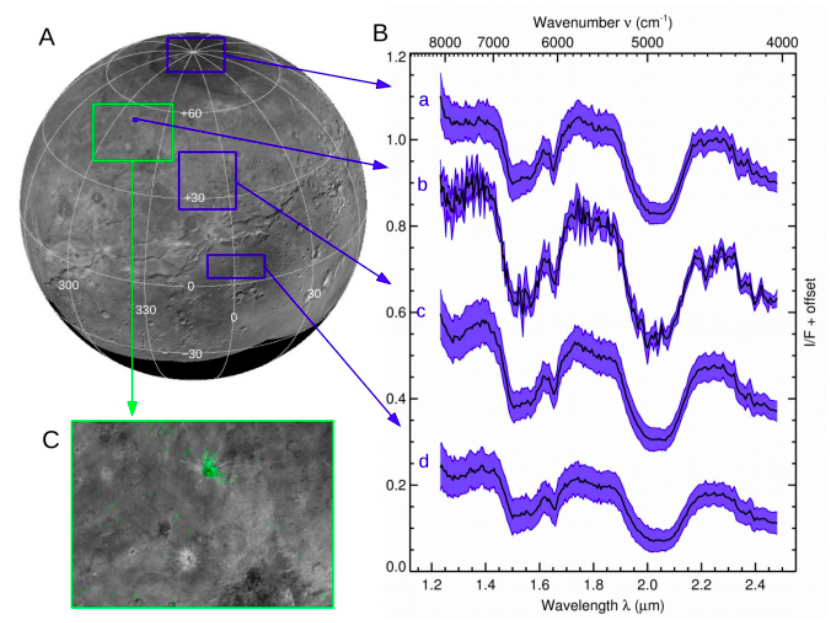
\includegraphics[width=\textwidth]{figures/chapter1/IR.png}
\caption{The 2.2$\mu$m absorption taken by LEISA camera colored as green on the topology shown by LORRI camera (A) and the spectra at 4 positions (B) with b taken near organa crater.(quoted from \cite{grundy2016surface})}
\label{fig:Charon_IR}
\end{figure}

Despite methane and ammonia, we still need energy to generate CN$^-$. In our solar system, there are many energetic sources, including solar wind, photons, cosmic rays from the outer solar system, etc. Among these, Ly-$\alpha$ photons appears to be the most important source in the dark side of Charon. It is attributed from sunlit(70 \%) and resonance scattering by atomic hydrogen flow (the excitment of electrons by hydrogen atoms and release ly-$\alpha$ photons in all directions)(30 \%) in the solar system \cite{grundy2016formation}. Its flux is $3.5 \times 10^7$ photons cm$^{-2}$ s$^{-1}$ at the winter pole of Charon \cite{grundy2016formation} which is 50 \% larger than expected before Mission New Horizons \cite{gladstone2015lyalpha}. We perform VUV irradiation on CH$_4$+NH$_3$ experiments with different ratios (including 3:2, 1:5, 1:10 and 1:20) to simulate the photon induced evolution on different concentrations of CH$_4$. The ratios in previous studies with electron irradiation experiments are CH$_4$ to NH$_3$ equals 3:1\cite{kim} and 3:2\cite{kundu2017electron}. As a complete study, we decided performing a ratio of CH$_4$ to NH$_3$ equals 3:2 to make possible comparisons.

\begin{figure}
\centering
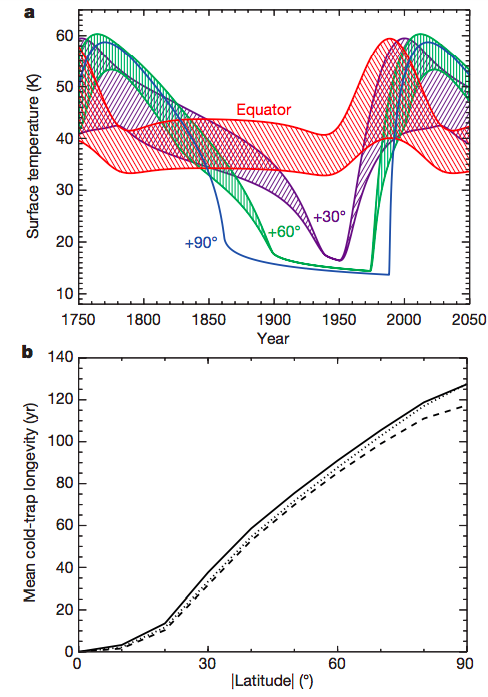
\includegraphics[width=0.5\textwidth]{figures/chapter1/thermal.png}
\caption{The temperature of Charon with thermal inertia 10 J m$^{-2}$ K$^{-1}$ s$^{-1/2}$ in 1750 to 2050 Earth years (a) and longest time the Latitude is under 25 K with the model averaged for 3 Myr with 2.5 (solid) 10 (dotted) and 40 (dashed) J m$^{-2}$ K$^{-1}$ s$^{-1/2}$ (b).(quoted from \cite{grundy2016formation})}
\label{fig:Charon_thermal}
\end{figure}

Apart from VUV irradiation, EUV irradiation also irradiates on Charon. The direct EUV irradiation (>12.4 eV) is $8.7 \times 10^7$ eV cm$^{-2}$ s$^{-1}$ at mean heliocentric distance 39 A.U. whereas VUV irradiation (Ly-$\alpha$ photons) is $1.9 \times 10^9$ eV cm$^{-2}$ s$^{-1}$ calculated by Grundy et al. (2016)\cite{grundy2016formation}. In order to investigate the effectiveness of EUV to VUV irradiation, we keep temperature of CH$_4$+NH$_3$ (3:2 \& 1:5) ice mixtures at 15 K and use the monochromatic 30.4 nm (40.8 eV) ,He II light provided by High flux beamline at National Synchrotron Radiation Research Centre (NSRRC) in Taiwan to irradiate the ice mixtures. The relative ratios of EUV irradiated ice is CH$_4$ to NH$_3$ = 3:2 and 1:5 for possible comparisons with VUV irradiations. \\

In this text, we will introduce the experimental methodology in chapter \ref{methods}, the formation mechanisms of main products of  EUV and VUV irradiated CH$_4$+NH$_3$ ice mixtures in chapter \ref{results}. With these results, we will know more details of Charon, especially the influences of photon sources. Different energy sources including electron irradiation experiments , EUV and VUV irradiations, and their astrophysical implications will be presented in chapter \ref{astron}.\\
               % 第一章    (自行寫入)
\chapter{\protect Methods}

\section{Laboratory Astrophysics}
To study the chemical reactivity in astrophysical environment experimentally,
we conducted our experiments in Interstellar photoprocessing system (IPS) (Chen et al. 2014),
an ultrahigh vacuum chamber with base pressure $3 \times 10^{-10}$ torr and 14 K,
corresponds to a density of $10^6$ cm$^{-3}$, similar to dense cloud interiors.
The system will be introduced in detail in section \ref{sec:IPS_system}.
To simulate the irradiation in interstellar environments,
we use a micro-wave discharge hydrogen lamp (MDHL) and monochromatic extreme-ultraviolet irradiation (EUV) 30.4 nm to irradiate our ice mixtures,
and they will be introduced in section \ref{sec:Vacuum_UV_source} and \ref{sec:Extreme_EUV_source} respectively.
The experimental protocols will be elaborated in section \ref{sec:Experimental_Protocol}.
In order to better understand the physics behind, some basic theories of Infrared spectroscopy and concepts of chemical kinetics used in data analysis are included in section \ref{sec:spectroscopy} and \ref{sec:Reaction_Rate_Laws} respectively.
To demonstrate the ice mixtures in KBOs, we used different configurations of ice mixtures that refers to different sections in chapter 3 and chapter 4.\\

\subsection{Experimental simulations by IPS system}
\label{sec:IPS_system}

We conducted our astrophysical simulations studied in chapter 3 to 4 in Interstellar Photo Processing System (IPS) (figure \ref{fig:system}). IPS consists in three systems: the main chamber, where our experiments take places; the detection system, where we collect our data; and a gasline system, where we prepare our samples.

\begin{figure}
\centering
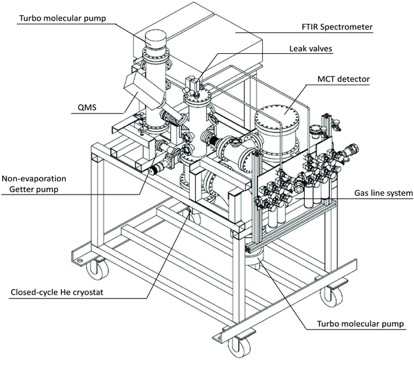
\includegraphics[width=\textwidth]{figures/chapter2/system.jpg}
\caption{The schematic diagram of IPS system, mechanical pumps are not shown for clarity. (Quoted from Chen et al. 2014)}
\label{fig:system}
\end{figure}

The main system consists of an ultrahigh vacuum chamber equipped with a closed-cycle helium cryostat (CTI-M350). It is pumped by a turbo molecular pump (KTKT FF – 160/620ZE, capacity 600 liters s$^{-1}$), which is backed up by a scroll pump, and a non –evaporation getter pump. The getter pump is a powerful tool to adsorb residue gases inside the main chamber, with a larger surface area, H$_2$, CO and N$_2$ are adsorbed to obtain a better base pressure. After baking, the base pressure of our main chamber can reach $1 \times 10^{-10}$ torr at 14 K, monitored by a Granville-Phillips 370 Stabil-Ion gauge. This pressure can be used to demonstrate the dense cloud interior environments and star forming region. The substrate we have chosen is KBr, which can allow infra-red photons with 700 to 4000 $cm^{-1}$ to penetrate. It is mounted by substrate holder made of oxygen-free copper, on the first stage of cold finger mounted on the tip of cryostat. Two silicon diodes and also a heater were placed onto the cold finger and one of the silicon diodes is near the substrate holder. They were connected to a temperature controller and PID system to achieve a warmup rate of 1K/min with an accuracy of 0.1 K.

The detection system consists in a mid-infrared Fourier transform spectrometer (mid-FTIR) (ABB FTLA2000-104) and a Quadrupole Mass Spectrometer (QMS). To prevent absorption bands of CO, CO$_2$ and H$_2$O gas in the atmosphere, the IR beam path was built inside vacuum, pumped by dry pump. The main chamber and the IR path are separated by ZnSe windows, which can allow infra-red penetration from 0.5 – 20 um with absorption less than 0.07 \%. In this study, the infrared spectra are obtained with resolution of 4 cm$^{-1}$ and averaged over 32 scans. The angle between the IR beam path and the substrate holder is 45 degrees. The QMS (MKS Microvision 2) consists of a controller and mechanical part sealed by a mounting flange in ultrahigh vacuum. It is mounted 10 cm from the substrate and run with a resolution 0.5 a.m.u. The Ionizer release 70 eV electron by filament and ionize incoming molecules to positive charged ions between anode grid and repeller. The ions were accelerated by focus plate and enters ion filter, which consists of four circular rods, with a combination of A.C and D.C. potential to sieve whole bandpass ions at millisecond timescale. The selected ions enter ion detector and are detected by either faraday cup and continuous dynode electron multiplier (CDEM) which can secondary multiply weak signals.

The samples are prepared in situ in our gasline system. It contains four stainless steel bottles with the same volume, which is used to determine relative proportion of the gas mixtures by their partial pressures. The ammonia gas 99.99 \% and methane 99.999 \% are mixed with partial pressure measured by a Baratron with 0 - 100 torr range with a 0.25% accuracy. The background pressure of the gasline system is lower than $1 \times 10^{-7}$ torr thank to a turbo molecular pump (Oerlikon Leybold TurboVac 151, capacity 145 liters s-1) backed up with an oil-sealed mechanical pump (Alcatel 2012A, capacity 450 $liters minute^{-1}$), equipped with an oil trap (molecular sieve type 13X). Water were bought from Merck which is LC-MS Grade and purified before use, by several freeze-pump-thaw cycles under vacuum.

\subsection{Vacuum-UV source}
\label{sec:Vacuum_UV_source}

In order to simulate the photoprocessing of vacuum ultraviolet (VUV) irradiation onto the interstellar ices and ices on planetary bodies, including KBOs, the ice mixtures are irradiated with a T-type Microwave-Discharged Hydrogen-flow lamp (MDHL). The molecular hydrogen with pressure 0.4 torr flows through the lamp with a support of a mechanical pump. Using a 2.4 GHz microwave generator and high voltage discharge, a low pressure plasma is produced in the Evenson cavity. Figure 2.2.1 shows a cross-section of T-type quartz tube; the middle part of the T-type quartz tube is being tunned by a ceramic rod that is called Evenson cavity.  In order to measure the photon flux in situ, we use an 88 \% transmittance nickel mesh with its photoelectric efficiency being obtained by high-flux beamline in National Synchrotron and a SXUV 100 photodiode calibrated by NIST. A MgF$_2$ window is placed between the lamp and the sample holder to prevent penetration of VUV photons with wavelength shorter than 114nm, leads to a cut off at 114nm. Figure 2.2.2 shows a VUV emission spectrum of a MDHL. It consists in Ly-α (121.6nm) and H$_2$ molecular emission in 110-180 nm range. Chen et al. (2014) showed that the spectral characteristics of the VUV light emitted in this range depends on the gas type (mixture of H$_2$ with He or Ar etc), pressure of H$_2$ and lamp geometry. Throughout those configurations stated there, we adopted 0.4 torr molecular hydrogen and T-type MDHL that produces VUV irradiation at 114-170 nm with 19.1 \% of Ly-α and a mean photon energy of 9.27 eV. The photon flux is $6.4 \times 10^{13}$ photons $cm^{-2} s^{-1}$ at sample position.


Figure 2.2.1 The cross-section of MDHL (T-type geometry) (Quoted from Chen et al. 2014).




Figure 2.2.2, VUV spectra of MDHL (T-type geometry, 110-180 nm) with different H$_2$ pressure inside the lamp(Quoted from Chen et al. 2014).

\subsection{Extreme EUV source}
\label{sec:Extreme_EUV_source}

To simulate the solar EUV irradiation reflected by IPM on both Charon and interstellar ices, we use the HF-CGM high – flux beam line of the National Synchrotron Radiation Research Center in Hsinchu, Taiwan. It provides a continuum EUV to VUV photons from 4 to 40 eV. The continuum is separated into monochromatic He II line (30.4nm) with a six-meter cylindrical grating monochrometer with an incident angle of 70 degrees. With the help of a movable entrance slit and movable curved exit slit, the energy resolving power can reach around $3 \times 10^4$ at 40 eV for grating 1600 l/mm with both slits movable and set opening to 10 $\mu m$ (Hsieh 1998). Similar to VUV irradiation provided by MDHL, the light intensity was monitored by the same nickel mesh with photoelectric efficiency obtained by SXUV 100 photodiode calibrated by NIST. With the known photoelectric efficiency, the flux of monochromatic 30.4nm is measured to be $2.15 \times 10^{14}$ photons $s^{-1} cm^{-2}$ with a spot size of 1 cm%^2% which is in the same order of magnitude of VUV continuum of MDHL. We replace the port with MDHL by the end station of the high-flux beamline. To prevent contaminations in the pipes and bellows, we placed a cryostat backed up by a scroll pump between our system and the beamline endstation. Between the cryostat and our main chamber is a SiO$_2$ valve, which is closed to prevent contamination to the end station during the warm-up phase.

\section{Experimental Protocol}
\label{sec:Experimental_Protocol}

In this section, we will briefly introduce the  procedures of how we performed our experiments. It is divided into four parts, preparation and cooling, deposition, irradiation and warmup.\\

Preparation of experiments and cooling\\
Before any of experiment is done, we bake our system at 100 oC for 48 hours to reduce the contamination of water and residue gases as much as possible. It was cooled to room temperature that the background pressure can reach routinely at $~ 1 \times 10^{-10}$ torr. The gasline were connected with the regulators of the gas tanks and bake to 100 $^oC$ and pumped by molecularturbo pump for two days before any experiment were done. Also, The water sample has been freeze thaw several times by liquid nitrogen until there is no pressure increase recorded by baratron when water is freezed. Before cooling the substrate to cryogenic temperature, we took an IR spectrum and started the monitoring of residue gases by QMS in order to compare the residue molecules and to verify any possible contaminations in the main chamber. We then start the cooling process thanks to the closed-cycle He cryostat.\\

Deposition\\
The gas mixtures are pre-mixed in our gasline system introduced in section \ref{sec:IPS_system}. We used a leak valve to condense the gas from the stainless steel bottles onto pre-cooled KBr substrate at 14 K, which monitored by Fourier transformed Infra-red spectroscopy (FTIR) and Quadrupole mass spectrometer (QMS) during deposition. The pressure of deposition is fixed to $1 \times 10^{-8}$ torr that the deposition rate is $4 \times 10^{16} molecules cm^{-2} min^{-1}$. After deposition, we placed the ice mixture at 14 K for 60 minutes and to allow pumping of residue gas, until pressure of the main chamber reduce back to its base pressure to simulate the interstellar environment before irradiation.\\

Photon Irradiation\\
The total irradiation time is 270 to 450 minutes depend on experiment configurations; with time intervals varies from 2 to 30 minutes. After each irradiation, we waited for 10 minutes allowing pumping out of the photodesorpted gas molecules. During irradiation, the photon flux is monitored by a nickel mesh. After Irradiation, we place the sample for 30 minutes to observe if any thermal reaction was conducted.\\

Warmup\\
We use 1 K/min to warmup the substrate to 300 K to demonstrate effects of a new born star nearby an interstellar cloud. During warmup, we record the QMS from 1 to 100 a.m.u. to observe if there are low quantity of higher mass product formed during irradiation.\\

\section{Infra-red spectroscopy and the Beer’s Law}
\label{sec:spectroscopy}
We used infra-red spectroscopy extensively in chapter 3 and 4, it is a powerful tool in studying molecular interactions during irradiation and warmup. We choose infra-red rather than Ramen spectroscopy because infra-red has lower energy that it would not change the structure of the ice mixture nor breaking any of the bonds. With different vibration modes, the energy absorbed by molecules are quantized. With the energy of absorption bands in infra-red spectrum, we may identify the functional group of the species. To simply classify, molecules can have, from less energetic, translational, rotational and vibrational motions. Generally, vibrational motions can be divided into stretching and bending. Stretching needs more energy than bending. For stretching, there exist Symmetric and Asymmetric stretching, while bending can be divided into In-plane Scissoring, rocking and out of plane Wagging and Twisting (Figure 2.4).\\

Figure 2.4 Different vibrational modes of a three atom molecule.
By Beer’s Law, we may calculate the column density of the molecule with its functional groups, which are used to plot figures in chapter 3 and 4. Beer Lambert’s Law suggest that when light passes through a medium, amount of light absorbed is proportional to density and path length of the medium. Assume the known intensity beam $I_{0}(\nu)$ passes through the medium and beam intensity become $I(\nu)$. The transmittance $T(\nu)$ is defined by equation \ref{eq:transmittance}. \\
\begin{equation}
T(\nu) = \frac{I(\nu)}{I_{0}(\nu)}
\label{eq:transmittance}
\end{equation}
Also, the absorbance $a(\nu)$ is defined by equation \ref{eq:absorbance}. \\
\begin{equation}
a(\nu) = - \ln T(\nu) = - \ln \frac{I(\nu)}{I_{0}(\nu)} = n l \sigma(\nu)
\label{eq:absorbance}
\end{equation}
where $n$ is number density (molecules/cm$^3$), $l$ is the path length (cm), $\sigma(\nu)$ is the cross-section (cm$^2$/molecule) of corresponding frequency $\nu$. This equation is known as Lambert Beer’s Law. \\

As the ice mixture in our thesis are at 14K, the peaks of absorbance are often a broadband due to coupling between neighbor molecules. Therefore, we can integrate the whole band of the peak equation \ref{eq:absorbance} with respect to frequency and use the absorbance strength (A value) in literatures to calculate the column densities $N$ of the ices by equation \ref{eq:column_density}.

\begin{equation}
N = \frac{\int a(\nu) \mathrm{d}\nu}{A(\nu)}
\label{eq:column_density}
\end{equation}
where $N$ is the column density (molecule cm$^{-2}$), $A(\nu)$ is the absorbance strength (cm molecule$^{-1}$).

\section{Reaction Rate Laws}
\label{sec:Reaction_Rate_Laws}
%In this section, we will introduce rate reaction of a consecutive reaction and the concept of pseudo first order which we used to fit our reaction product against irradiation time. The rate of a chemical reaction is the relation between change in concentration of a substance per unit of time. i.e. For  a balanced chemical reaction, A → 2B, the rate of reaction is . The formation rate of B is 2 times destruction rate of A.

%When there are two reactants, with balanced equation 2 A + B → 2C. The reaction is a third order overall, second order in A and first order in B. rate = k [A]2[B].

%To determine the order of a reaction, we can only determine it experimentally. One way is method of initial rates. By changing concentration of initial reactants, and find out the initial reaction rate, we may find out the relation between two reactants and the rate. i.e. Rate=k[A]x[B]y.
%For a reaction with only one reactant [R], we may use the relation between time and reactant concentration to plot graphs to find out the order or reaction.
%For a zero order reaction, the rate is not depending on any reactant that it is a constant. The Rate =  .By calculus, .
%For a first order reaction,  . By calculus ln[R]t = -k t +ln [R]0
%For a second order reaction,  . By calculus.
%Hence, if we get a straight line in a plot between time as x-axis, and the concentration of reactant as y axis, it is a zeroth order reaction, similarly, in first order reactions, we get straight line in plots between ln[R] as y axis and t in x axis.

%In a reaction with one reactant in excess, the rate of reaction is called pseudo first order reaction where Pseudo means pretended. For A+B → C, rate = k [A][B]. As [B]o>>[A]o, change of [B] is negligible that [B] ~ [B]o. Therefore, [B] is assumed to be a constant and included in the rate constant k.

%For a consecutive reaction, where A → B → C that the produced product will not convert back as reactant. A simple example is radioactive decay. At t=0,  [A]=[A]o, [B]=0, [C]=0 and at all times, [A]+[B]+[C]=[A]o.  The rate equations are as follows:



%By equation (2.4), we get
%subsitute into equation (2.5), we get B]=, by solve differential equation, we get equation (2.6).

%Finally, since [C]=[A]o-[B]-[A], by equation (2.7), we get


%Since the ratio of CH4 and NH3 are 3:2, 1:5, 1:10 and 1:20, hence, we may apply pseudo first order. By Kim & Kaiser (2011), B is the intermediate methylamine CH3NH2.
%We may use consecutive reaction equation 2.8 to fit the product CN- because there are no obvious peaks at 2200cm-1 that there is no destructive pathway of CN-.
               % 第二章    (自行寫入)
\chapter{\protect Results and Discussions}
\label{results}
According to the New Horizons team \cite{grundy2016formation}, CH$_4$ from Pluto may accumulate onto the surface of Charon by cold-trapping. The amount of CH$_4$ varies along the surface of Charon because it depends on the length of time the temperature is below 25 K which in turns depends on diurnal motion and thermal inertia of Charon. With an axis tilted by 112 degrees from the ecliptic, higher concentration of CH$_4$ will be accumulated at the pole (see chapter \ref{introduction} for details). In this chapter, we will investigate the following by infra-red spectroscopy: 1. The photo products produced by different concentration ratios of methane to ammonia, 2. the photo products produced by different photo sources (i.e. EUV and VUV) 3. the reaction mechanisms of each main products and 4. the functional group of tholin formed by irradiation of VUV, EUV on different configurations of CH$_4$+NH$_3$ ice mixtures (the result is compared with the residues on Titan produced by Imanaka et al. \cite{imanaka2004laboratory}).

\section{The infra-red spectrums and peaks identification}
We scanned the IR spectrum before and after deposition and plotted the plot the corresponding absorbance of the ice mixtures. Figure \ref{fig:widerange} is a plot of the absorbance of the CH$_4$+NH$_3$ ice mixtures in different concentration ratios: 1:20, 1:10, 1:5 and 3:2 ( arrangedfrom top to bottom). We label the peaks used in column density calculation  by dotted lines in  the graph. Main products we have detected are C$_2$H$_6$, CN$^-$ and C$_3$H$_8$. The peak positions for substance identification are listed in Table \ref{tab:WavenumberMDHL}. After identification of the products, we will look into each main products individually.\\

\begin{figure}
\centering
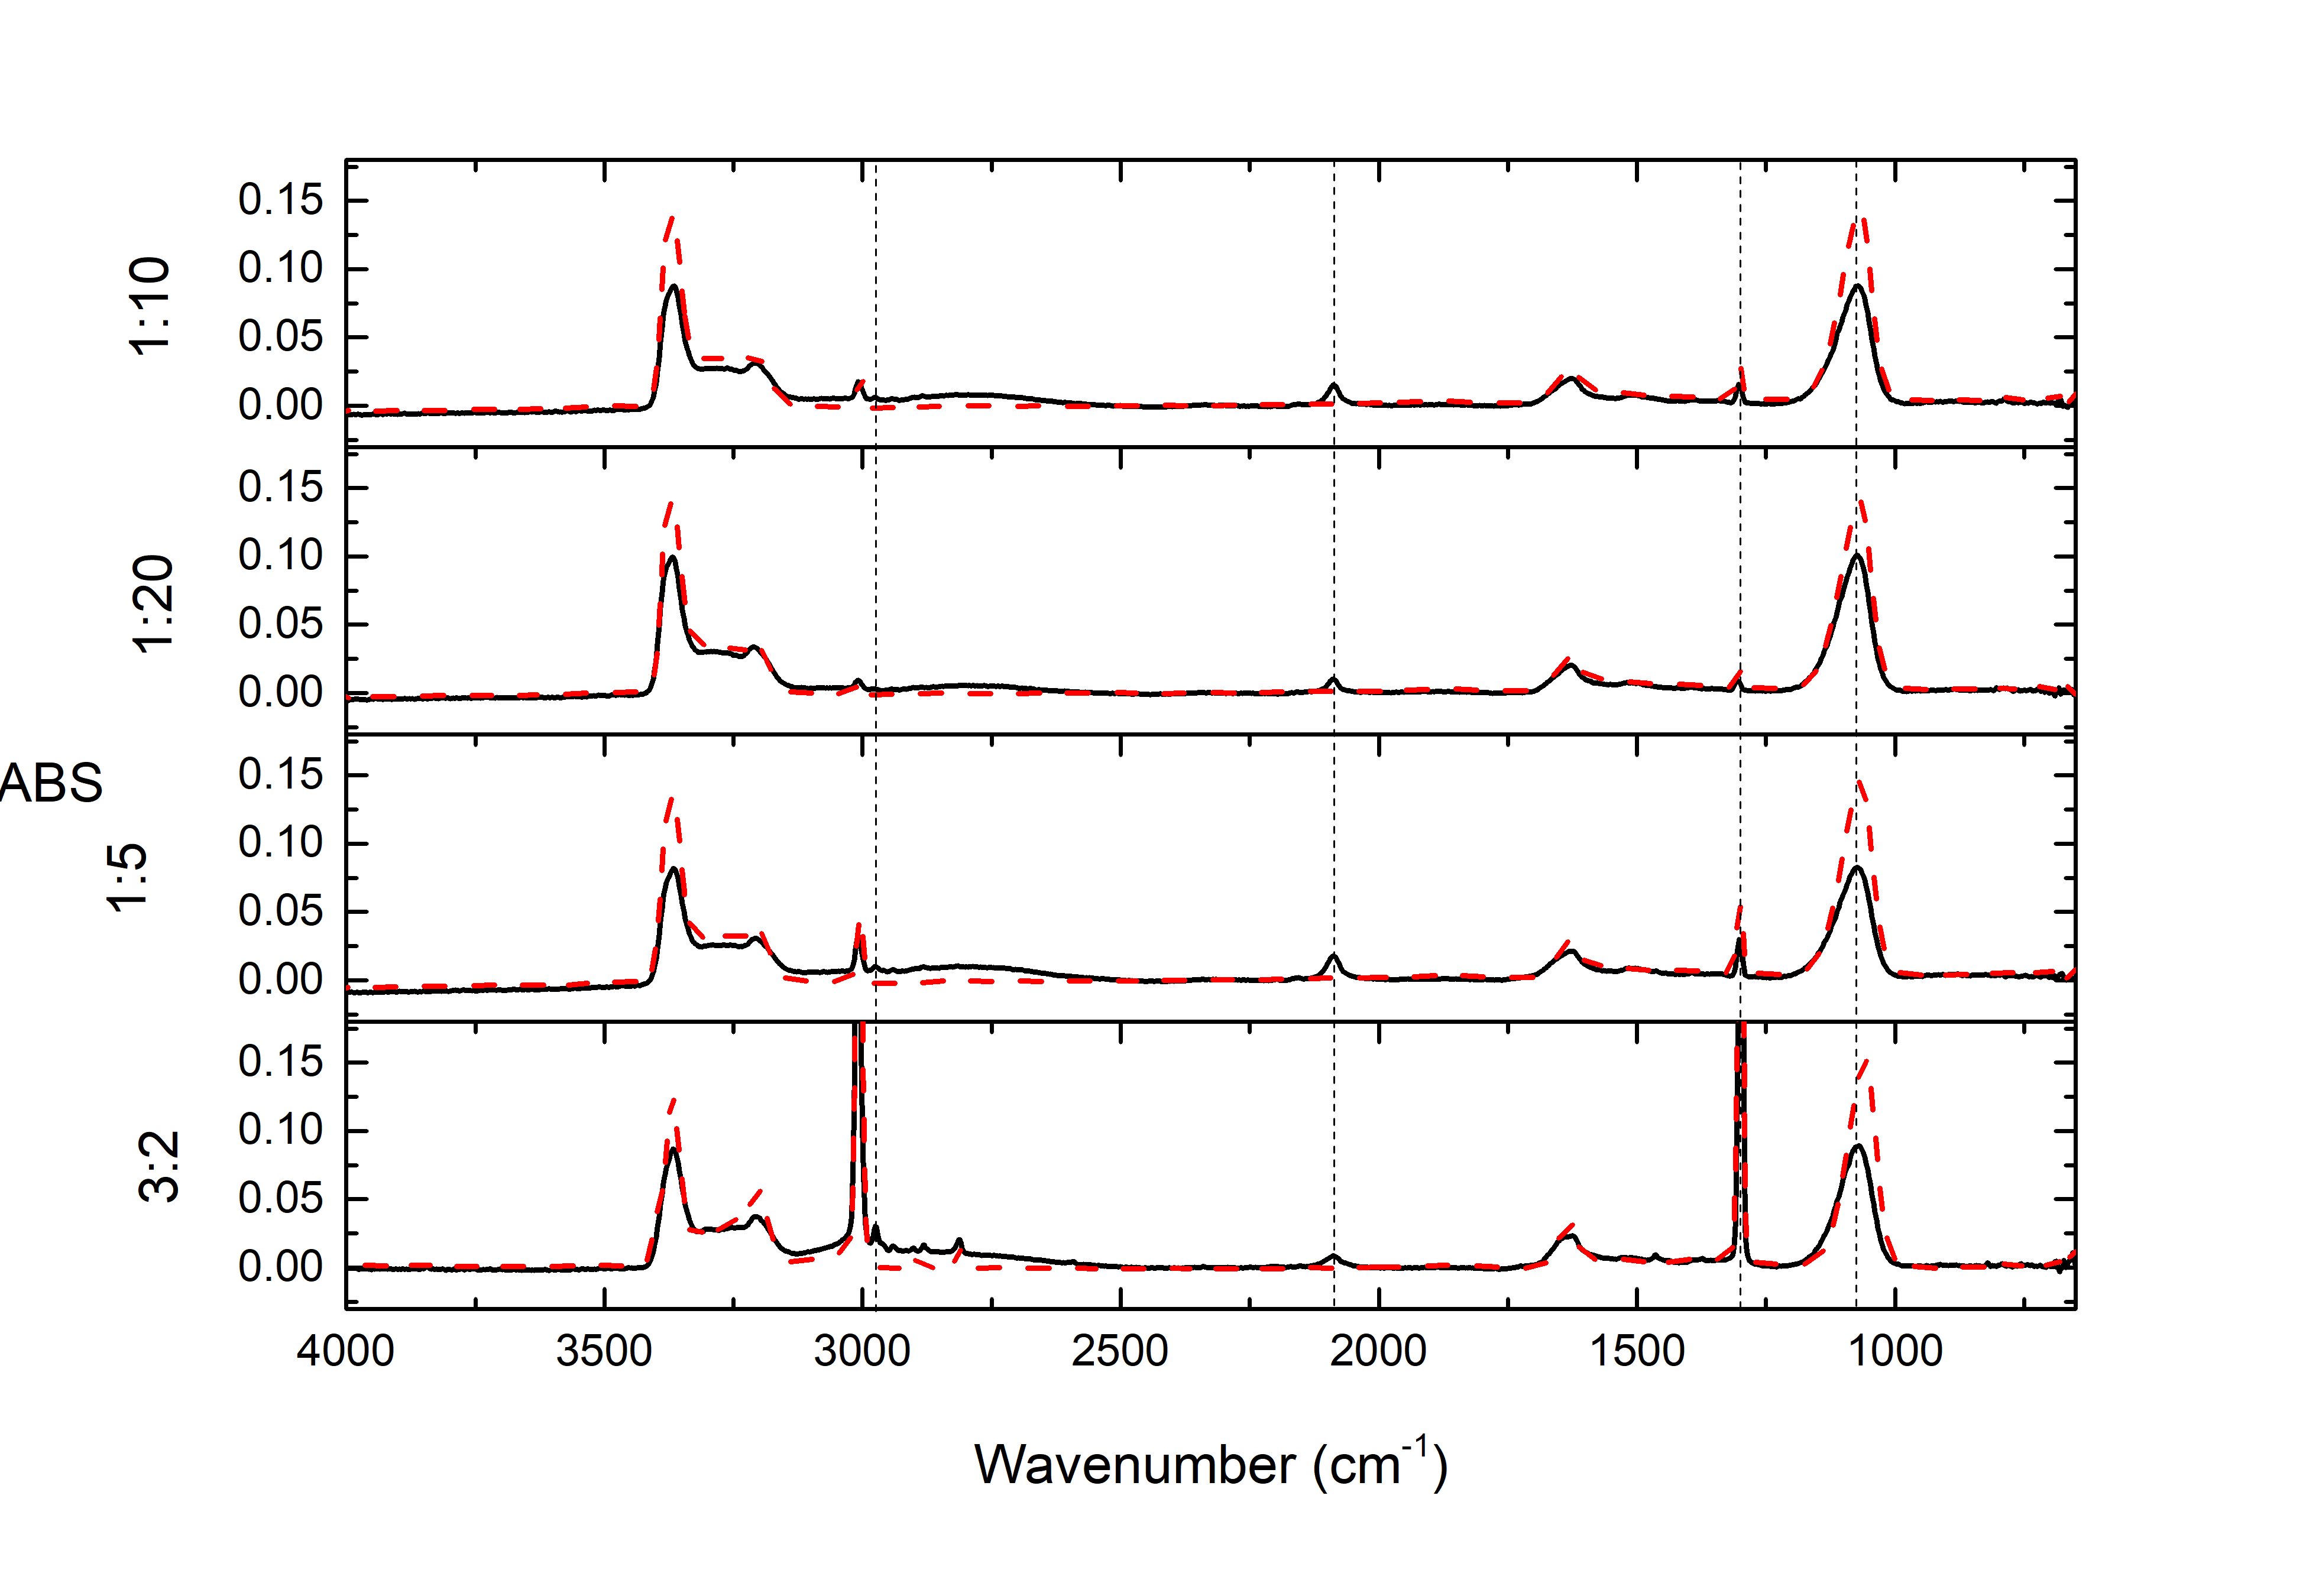
\includegraphics[width=\textwidth]{figures/chapter3/widerange.png}
\caption{The the infra-red spectrum of CH$_4$ + NH$_3$ ice mixtures before irradiation (dashed) and VUV irradiated ice mixtures provided by MDHL. }
\label{fig:widerange}
\end{figure}

\begin{table}[htbp]
\caption{The peak positions of identified substances after irradiation in different configurations of ice mixtures.}
\label{tab:WavenumberMDHL}
\begin{tabular}{ccccccc}
\hline
\hline
\multicolumn{2}{c}{Literture assignments} & \multicolumn{4}{c}{CH$_4$+NH$_3$ ratio (MDHL)} &  \\
\hline
Wavenumber & Carrier  & 1:5  & 1:10  & 1:20  & 3:2  & Ref. \\
(cm$^{-1}$) &   & (cm$^{-1}$) & (cm$^{-1}$) & (cm$^{-1}$) & (cm$^{-1}$) &\\
\hline
3375 & $\nu_3$ (NH$_3$) & 3366 & 3366 & 3369 & 3367 & 1 \\
3290 & $2\nu_4$ (NH$_3$) & - & - & - & - & 1 \\
3210 & $\nu_1$ (NH$_3$) & 3207 & 3208 & 3210 & 3205 & 1 \\
3011 & $\nu_3$ (CH$_4$) & - & - & - & - & 2 \\
2972 & $\nu_{10}$ (C$_2$H$_6$) & 2975 & - & - & 2975 & 3 \\
2960 & C$_3$H$_8$ & - & - & - & 2960 & 7 \\
2941 & $\nu_8+\nu_11$ (C$_2$H$_6$) & 2940 & - & - & 2940 & 3 \\
2904 & $\nu_1$ (CH$_4$) & 2901 & - & - & 2901 & 5 \\
2879 & $\nu_5$ (C$_2$H$_6$) & 2882 & 2883 & - & 2882 & 3 \\
2814 & $\nu_2+\nu_4$ (CH$_4$) & - & - & - & 2815 & 5 \\
2083 & $\nu$ (CN$^-$) & 2088 & 2087 & 2088 & 2088 & 2 \\
1625 & $\nu_4$ (NH$_3$) & 1625 & 1625 & 1626 & 1631 & 1 \\
1514 & $\delta$ (NH$_2$) & 1509 & 1507 & 1505 & 1511 & 6 \\
1465-1440 & deform CH$_2$ scissor & 1461 & - & - & 1463 & 3,4 \\
1390-1370 & CH$_3$ sym deform & 1394 & 1394 & 1394 & 1372 & 4 \\
1298 & $\nu_4$ (CH$_4$) & 1301 & 1302 & 1305 & 1299 & 2 \\
1075 & $\nu_2$ (NH$_3$) & 1073 & 1072 & 1072 & 1072 & 1 \\
820 & $\nu_12$ (C$_2$H$_6$) & - & - & - & 820 & 3 \\
\hline
\end{tabular}\\
Reference: 1. Bossa et al. 2008 \cite{bossa2008carbamic} 2. Moore and Hudson 2003 \cite{moore2003infrared} 3. Kim et al. 2010 \cite{kim2010abiotic} 4. Socrates 2001 \cite{socrates2001infrared} 5. Bennet and Kaiser 2007 \cite{bennett2007formation} 6. Zheng et al. 2008 \cite{zheng2008formation} 7. Hudson and Moore 2004 \cite{hudson2004reactions}
\end{table}



To calculate the column density, we integrate the area under graph and divide it by the absorption strength presented in table 3.2. We aware that there is an average error in absorption strengths of no more than 10 \%  when the pure ice is diluted in N$_2$ and H$_2$O \cite{richey2012near}. In our case, absorption strengths changes after CH$_4$ and NH$_3$ are mixed. For example, according to d' Hendecourt and Allamandola \cite{d1986time}, the band of NH$_3$ located at 1070 cm$^{-1}$ would not change much (from $1.1 \times 10^{-17}$ to $1.2 \times 10^{-17}$) when excess water is added to pure NH$_3$. For the case of CN$^-$, we know that CN$^-$ has a bond order =3 from its molecular orbitals. CN$^-$ is different from CN (bond order 2.5).  CN stretching is very sensitive to the matrix environment. It can change by factor of 2 in amino acetonitrile and H$_2$O (1:3) \cite{borget2012aminoacetonitrile}. However, CN is not inspected in this chapter. Therefore, we are justified to use the same absorption strength throughout our discussion to estimate the column density of each species and how the absorption area changes with concentration ratios of ice mixtures and photon energy. Here, we adopt the absorption strengths stated in Table \ref{tab:Absorbance} \\

\begin{table}[htbp]
\caption{The strength of absorbance adopted in this thesis measured in literatures of pure ice samples}
\label{tab:Absorbance}
\begin{tabular}{cccccc}
\hline
\hline
Wavenumber (cm$^{-1}$) & Assignment  & Vibration & FWHM & A value ($\times 10^{-17}$) & Reference \\
\hline
2976 &  C$_2$H$_6$ & -CH$_3$ & - & 1.05 & 2 \\
2960 & C$_3$H$_8$ & -CH$_2$- & - & 2.58 & 2 \\
2086 & CN$^-$ & CN & - & 1.8 & 3 \\
1297 & CH$_4$ & CH deformation & 8 & 0.61 & 1 \\
1070 & NH$_3$ & "umbrella mode" & 68 & 1.7 & 1 \\
\hline
\end{tabular}
Reference: 1. d'Hendecourt and Allamandola (1986)\cite{d1986time} 2. Moore and Hudson (1998)\cite{moore1998infrared} 3. Noble et al. (2013) \cite{noble2012thermal}
\end{table}


\section{Reaction mechanisms} %mechanisms

\subsection{C$_2$H$_6$}

\begin{figure}
\centering
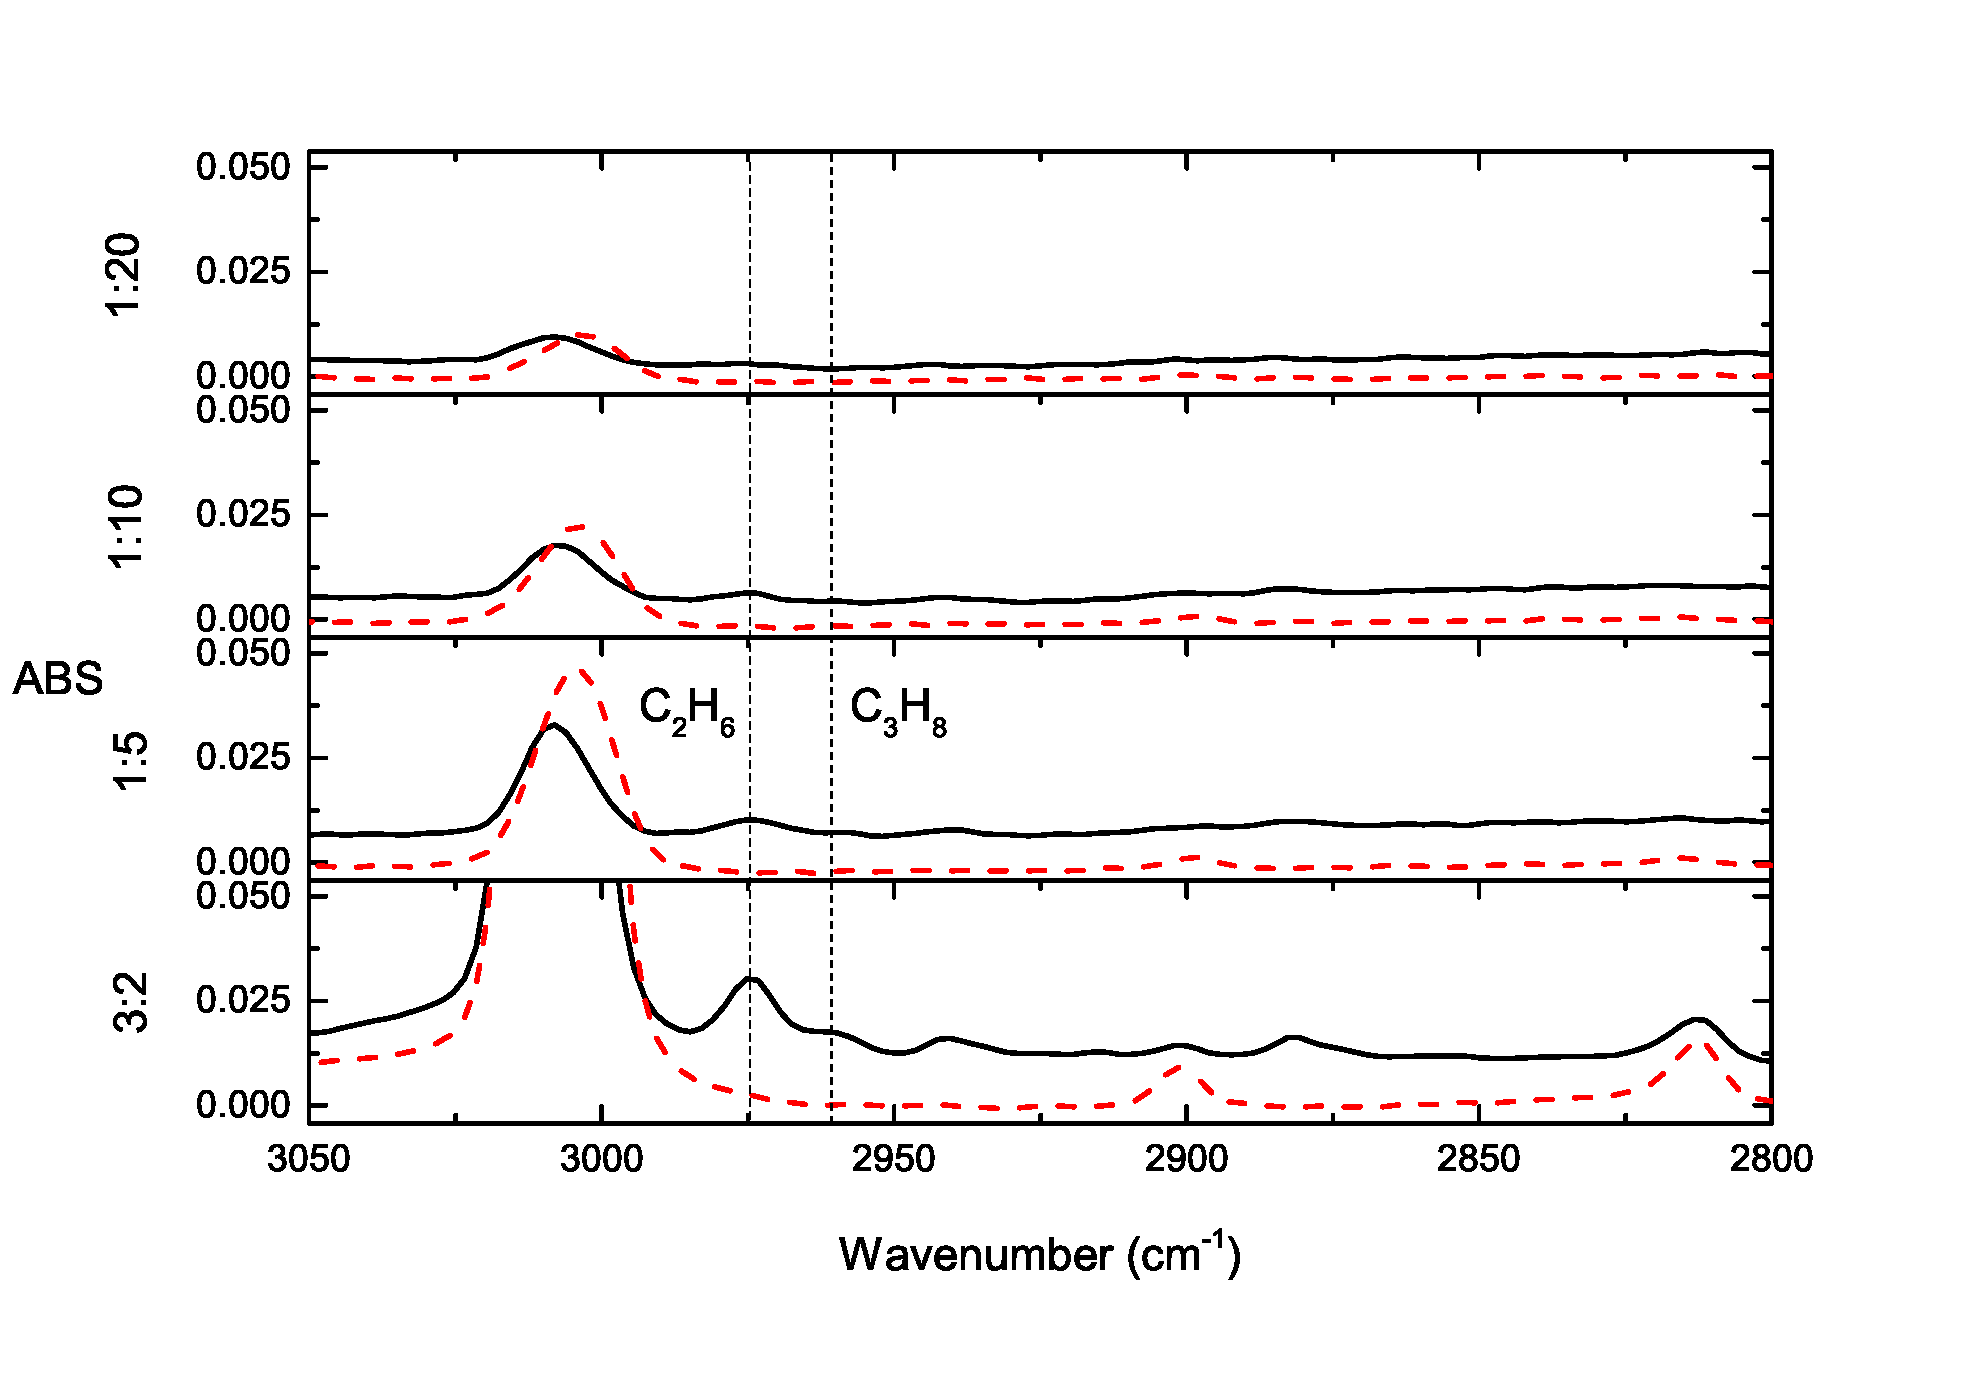
\includegraphics[width=\textwidth]{figures/chapter3/C2H6.eps}
\caption{The the infra-red spectrum of CH$_4$ + NH$_3$ ice mixtures of C$_2$H$_6$ and C$_3$H$_8$ before irradiation (dashed) and VUV irradiated ice mixtures provided by MDHL. }
\label{fig:C2H6}
\end{figure}

The assignment of C$_2$H$_6$ is confirmed by several bands listed in table \ref{tab:WavenumberMDHL}. Figure \ref{fig:C2H6} is a zoomed view of figure \ref{fig:widerange}. The absorption peak located at 2075 cm$^{-1}$ corresponds to the strongest vibration of C$_2$H$_6$. The formation of C$_2$H$_6$ in astrophysical environment is mainly a combination with 2 CH$_3$ radicals \cite{bennett2006laboratory}:

\begin{equation}
CH_4 + hv \rightarrow CH_3
\label{eq:CH3}
\end{equation}
\begin{equation}
2 CH_3 \rightarrow C_2H_6
\label{eq:C2H6}
\end{equation}

The energy required to produce 1 CH$_3$ radical from CH$_4$ is 4.42 eV.  Recombination of 2 CH$_3$ radicals forms C$_2$H$_6$ releases 3.74 eV. The process in \ref{eq:C2H6} is a no-barrier exothermic process. Note that C$_2$H$_6$ is not detected in CH$_4$ to NH$_3$=1:20 ice mixtures. Figure \ref{fig:lab_C2H6} shows the temporal formation column density of C$_2$H$_6$ in different configurations of irradiated ice mixtures.  As the formation only depends on CH$_4$, we may use first order kinetics equation to fit the column density versus photon dose.

\begin{equation}
[A] = [A]_0(1 - e^{-k_1 t})
\label{eq:1step}
\end{equation}
The fitting results are shown in table \ref{tab:fittingC2H6}.

\begin{figure}
\centering
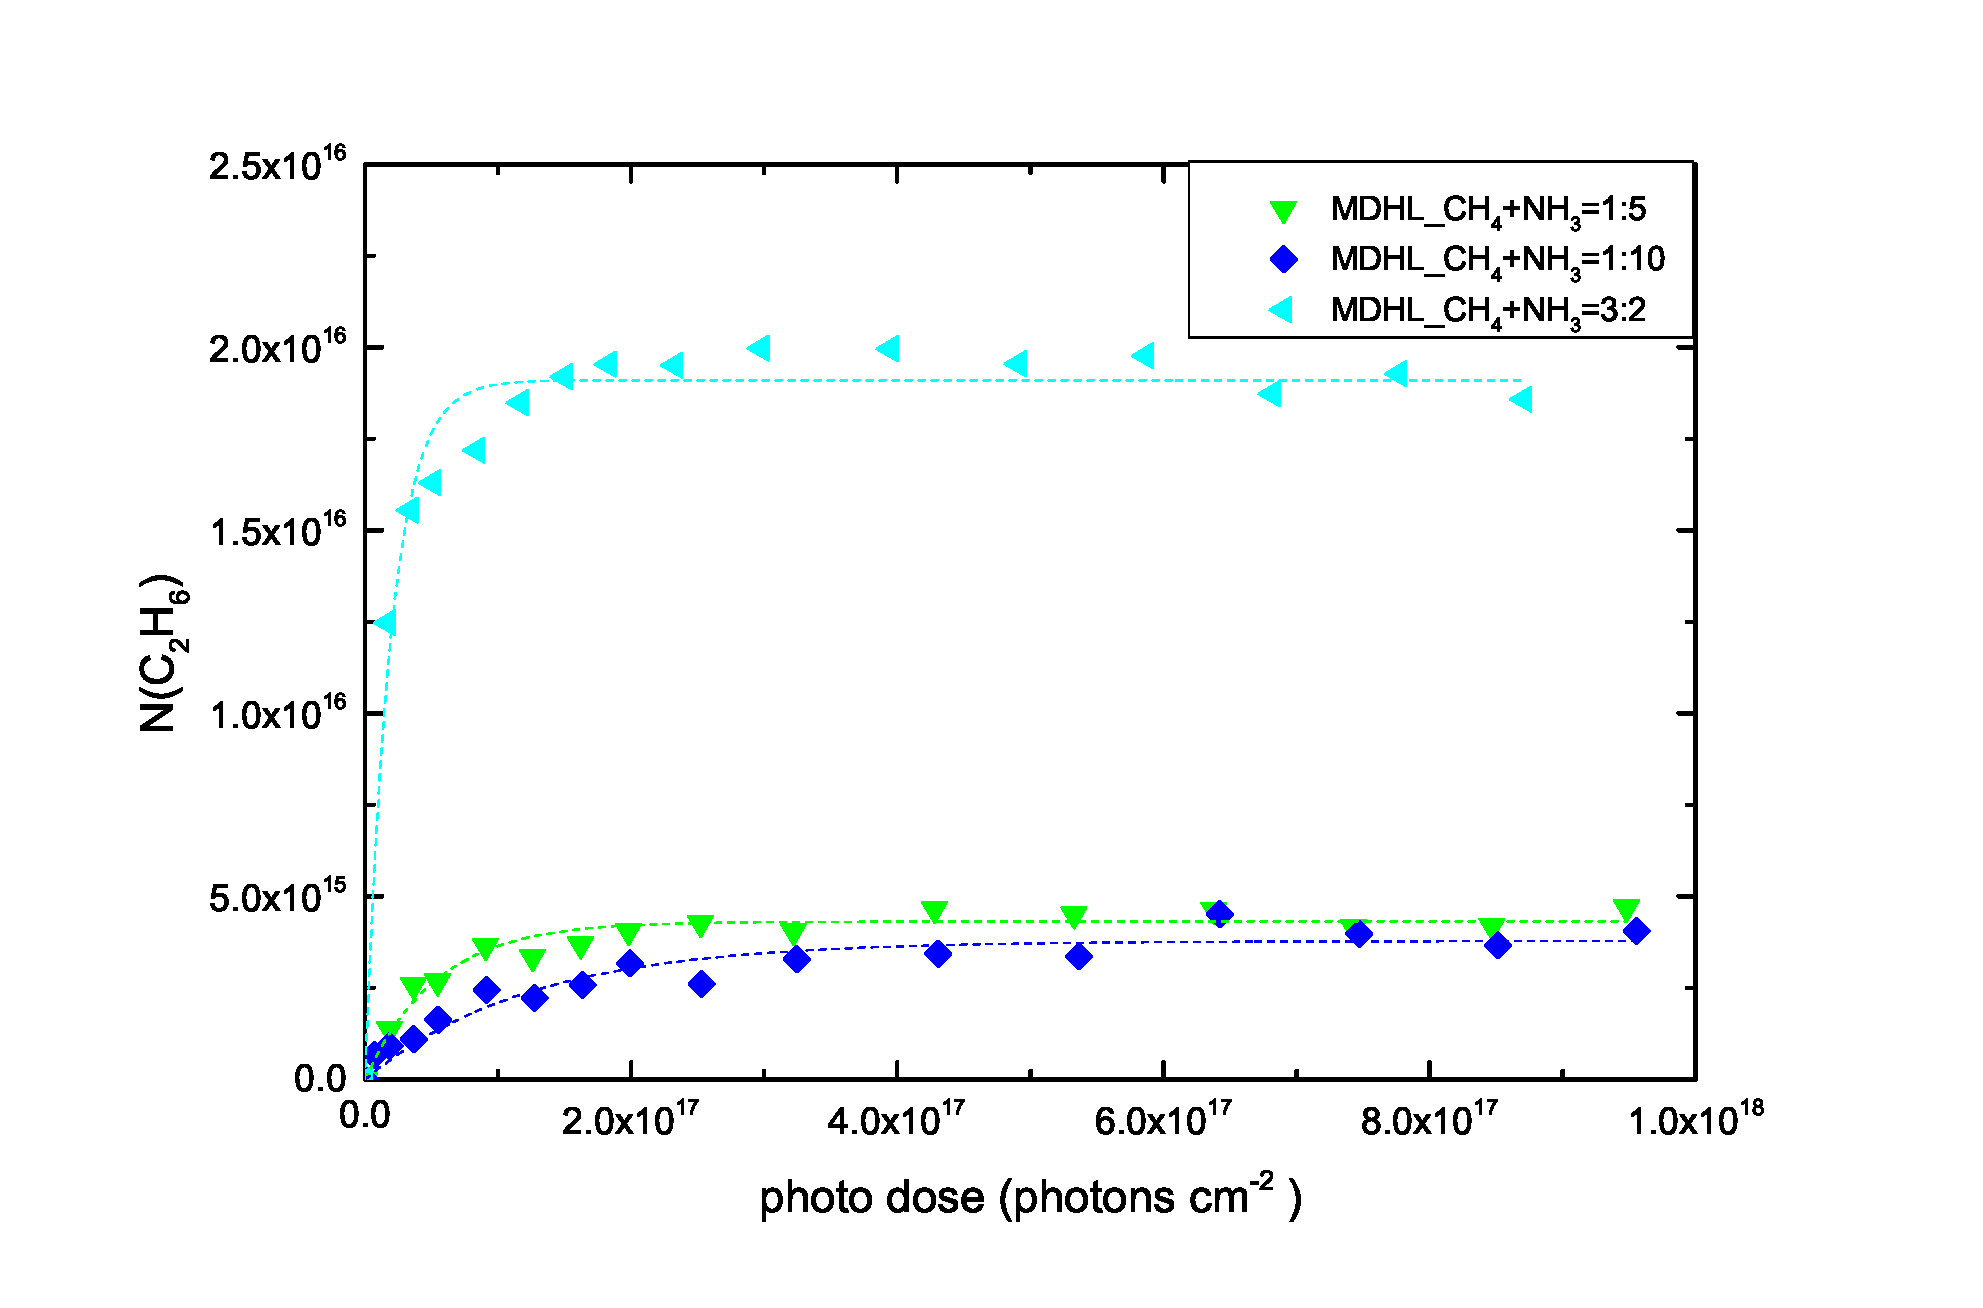
\includegraphics[width=\textwidth]{figures/chapter3/Lab_C2H6.eps}
\caption{The column density of C2H6 during CH4 + NH3 ice mixtures irradiated by MDHL. }
\label{fig:lab_C2H6}
\end{figure}

\begin{table}[htbp]
\caption{The fitting results of C$_2$H$_6$ by [C$_2$H$_6$]=[C$_2$H$_6$]$(1 - e^{-k_1 t})$}
\label{tab:fittingC2H6}
\begin{tabular}{ccc}
\hline
\hline
Ratio of CH$_4$+NH$_3$ & A (x10$^{15}$ molecules cm$^{-2}$) & k (x10$^{-17}$ photon$^{-1}$) \\
\hline
1:10 & 2.90 $\pm$ 1.25 & 0.92 $\pm$ 0.15 \\
1:5 & 4.16 $\pm$ 0.28 & 2.28 $\pm$ 0.28 \\
3:2 & 19.2 $\pm$ 0.15 & 5.28 $\pm$ 0.25 \\
\hline
\end{tabular}
\end{table}

From table \ref{tab:fittingC2H6}, the production rate is nearly proportional to the initial CH$_4$ concentration.


\subsection{C$_3$H$_8$}

The peak positioned at 2960 cm$^{-1}$ belongs to -CH$_2$- so we assign that as C$_3$H$_8$, as the shortest carbon chain. The signal to noise ratio in CH$_4$+NH$_3$ = 1:10 is poor that we can not quantize the amount of C$_3$H$_8$ (figure \ref{fig:C2H6}).

It is a secondary product formed by a combination of either C$_2$H$_6$ + CH$_2$ (equation \ref{eq:C3H81})or C$_2$H$_4$ + CH$_4$ (equation \ref{eq:C3H82}).
\begin{equation}
C_2H_6 + CH_2 \rightarrow C_3H_8
\label{eq:C3H81}
\end{equation}
\begin{equation}
C_2H_4 + CH_4 \rightarrow C_3H_8
\label{eq:C3H82}
\end{equation}

By modern peak fitting method, we deconvolute the overlapped C$_2$H$_6$ and C$_3$H$_8$ into two gaussians.

\subsection{CN$^-$}

\begin{figure}
\centering
\includegraphics[width=\textwidth]{figures/chapter3/CN.eps}
\caption{The infra-red spectrum of CH$_4$ + NH$_3$ ice mixtures of C$_2$H$_6$ and C$_3$H$_8$ before irradiation (dashed) and VUV irradiated ice mixtures provided by MDHL. }
\label{fig:CN}
\end{figure}

From infra-red absorption spectrum (figure \ref{fig:CN}) and their positions, we assign the peak 2086 cm$^{-1}$ to CN$^-$  but not a combination of HCN and CN$^-$. The assignment is based on a absence in CN bending mode at 848 cm$^{-1}$. In the case CH$_4$ + NH$_3$ = 3:2, we may observe a peak located at 820 cm$^{-1}$, which is with a FWHM half of HCN and it is eliminated at 50 K during the warm-up phase. Since 50 K is the desorbing temperature of C$_2$H$_6$ and the peak position is close to $\nu$12 mode of C$_2$H$_6$, we believe that the 820 cm$^{-1}$ peak is contributed by C$_2$H$_6$. Therefore, we may assign our peak located at 2086 cm$^{-1}$ as purely CN$^-$.\\

\begin{figure}
\centering
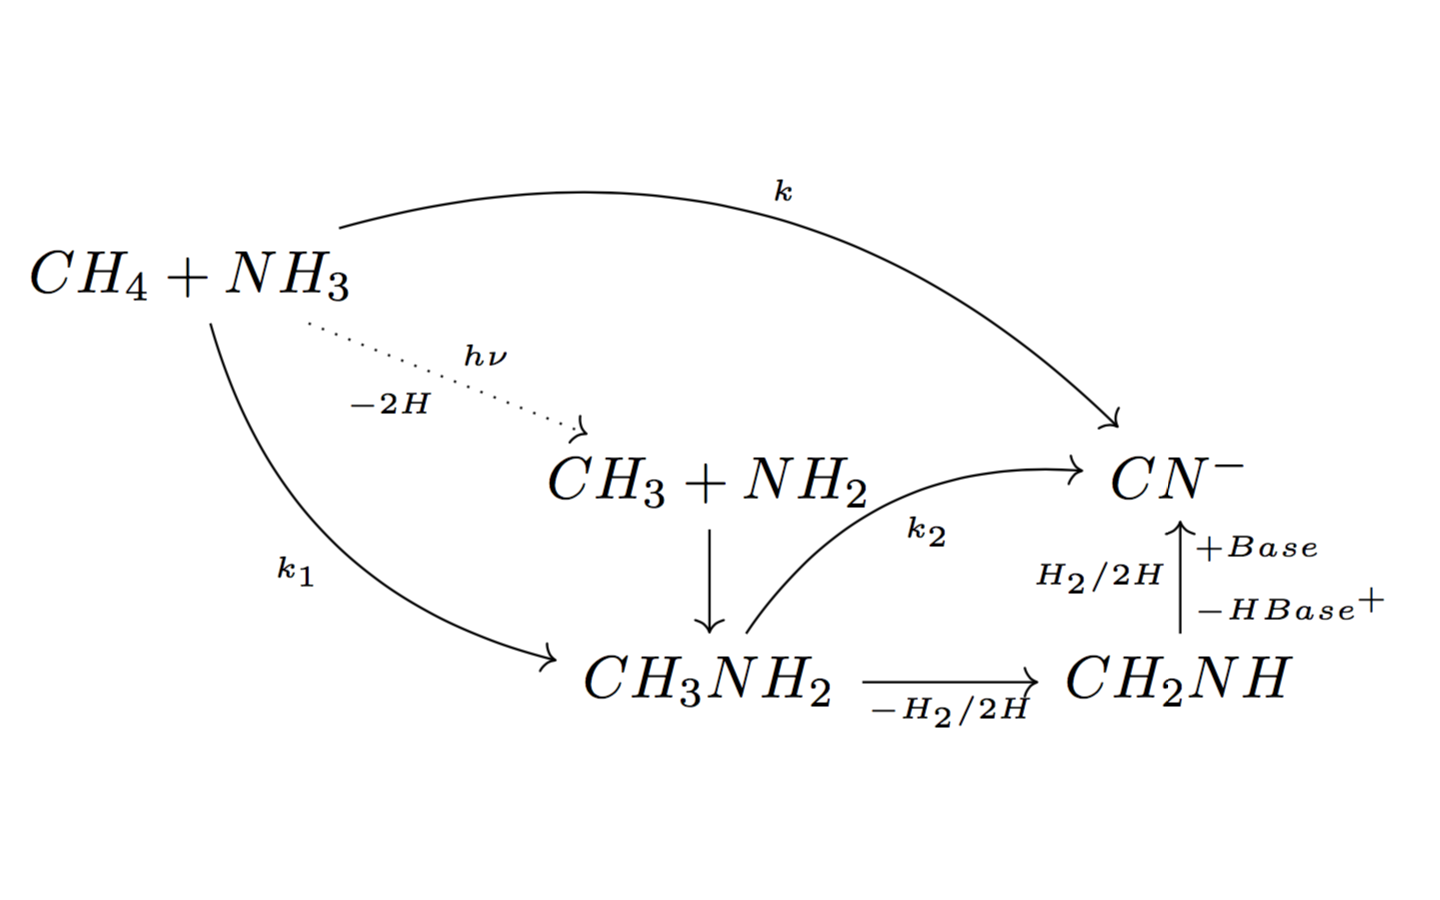
\includegraphics[width=\textwidth]{figures/chapter3/CNmechanism}
\caption{The formation mechanism of CN$^-$ proposed by Kim and Kaiser(2011)\cite{kim} .}
\label{fig:CNmechanism}
\end{figure}

The formation mechanism of CN$^-$ at low temperature was first suggested by Kim and Kaiser (2011) \cite{kim} to be two step reaction mechanism with methylamine as intermediate. CH$_4$ and NH$_3$ irradiated by photon become CH$_3$ and NH$_2$ radicals (figure \ref{fig:CNmechanism}), followed by propagation and recombination of radicals becoming CH$_3$NH$_2$ and dehydrogenation and acid-base reaction to form CN$^-$.
Although Kim and Kaiser (2011) \cite{kim} used 1.5 keV electron as energy source to simulate the cosmic ray induced photochemistry, this formation mechanism also applies in our photon irradiation experiments because we can also detect the methylamine during our warm-up phase. The ion fragment with m/z=31 is assigned as CH$_3$NH$_2$$^+$ and detectable in all ratios of our CH$_4$+NH$_3$ experiments (figure \ref{Mass31}).

\begin{figure}
\centering
\includegraphics[width=\textwidth]{figures/chapter3/Mass31.eps}
\caption{The m/z=31 detected by QMS during warm-up with heating rate 1 K/min in different configurations of ice mixtures.}
\label{Mass31}
\end{figure}

By the deviation perform in section \ref{sec:Reaction_Rate_Laws}, we have a rate equation for consecutive reactions \ref{eq:rate7}. With one of the reactant larger than another, we apply the pseudo first order assumption. With equation \ref{eq:rate7}, we fit the formation of CN$^-$ (figure \ref{fig:CNrate})and find that one of the rate constant is always larger than the other in all of the ratios. The fitting results are averaged by more than two experiments and are shown in table \ref{tab:CNrate}.The results of Kim and Kaiser is also listed into the table, they could observe a two-step reaction mechanism in production of CN$^-$ in CH$_4$+NH$_3$ (3:1) experiments with electron current 0.1 $\mu$A. However, when they increase the electron flux to 1 $\mu$A for irradiation C$_n$H$_{2n+2 (n=1-6)}$ and NH$_3$ ice mixtures, they also observe a one-step reaction mechanism.

\begin{figure}
\centering
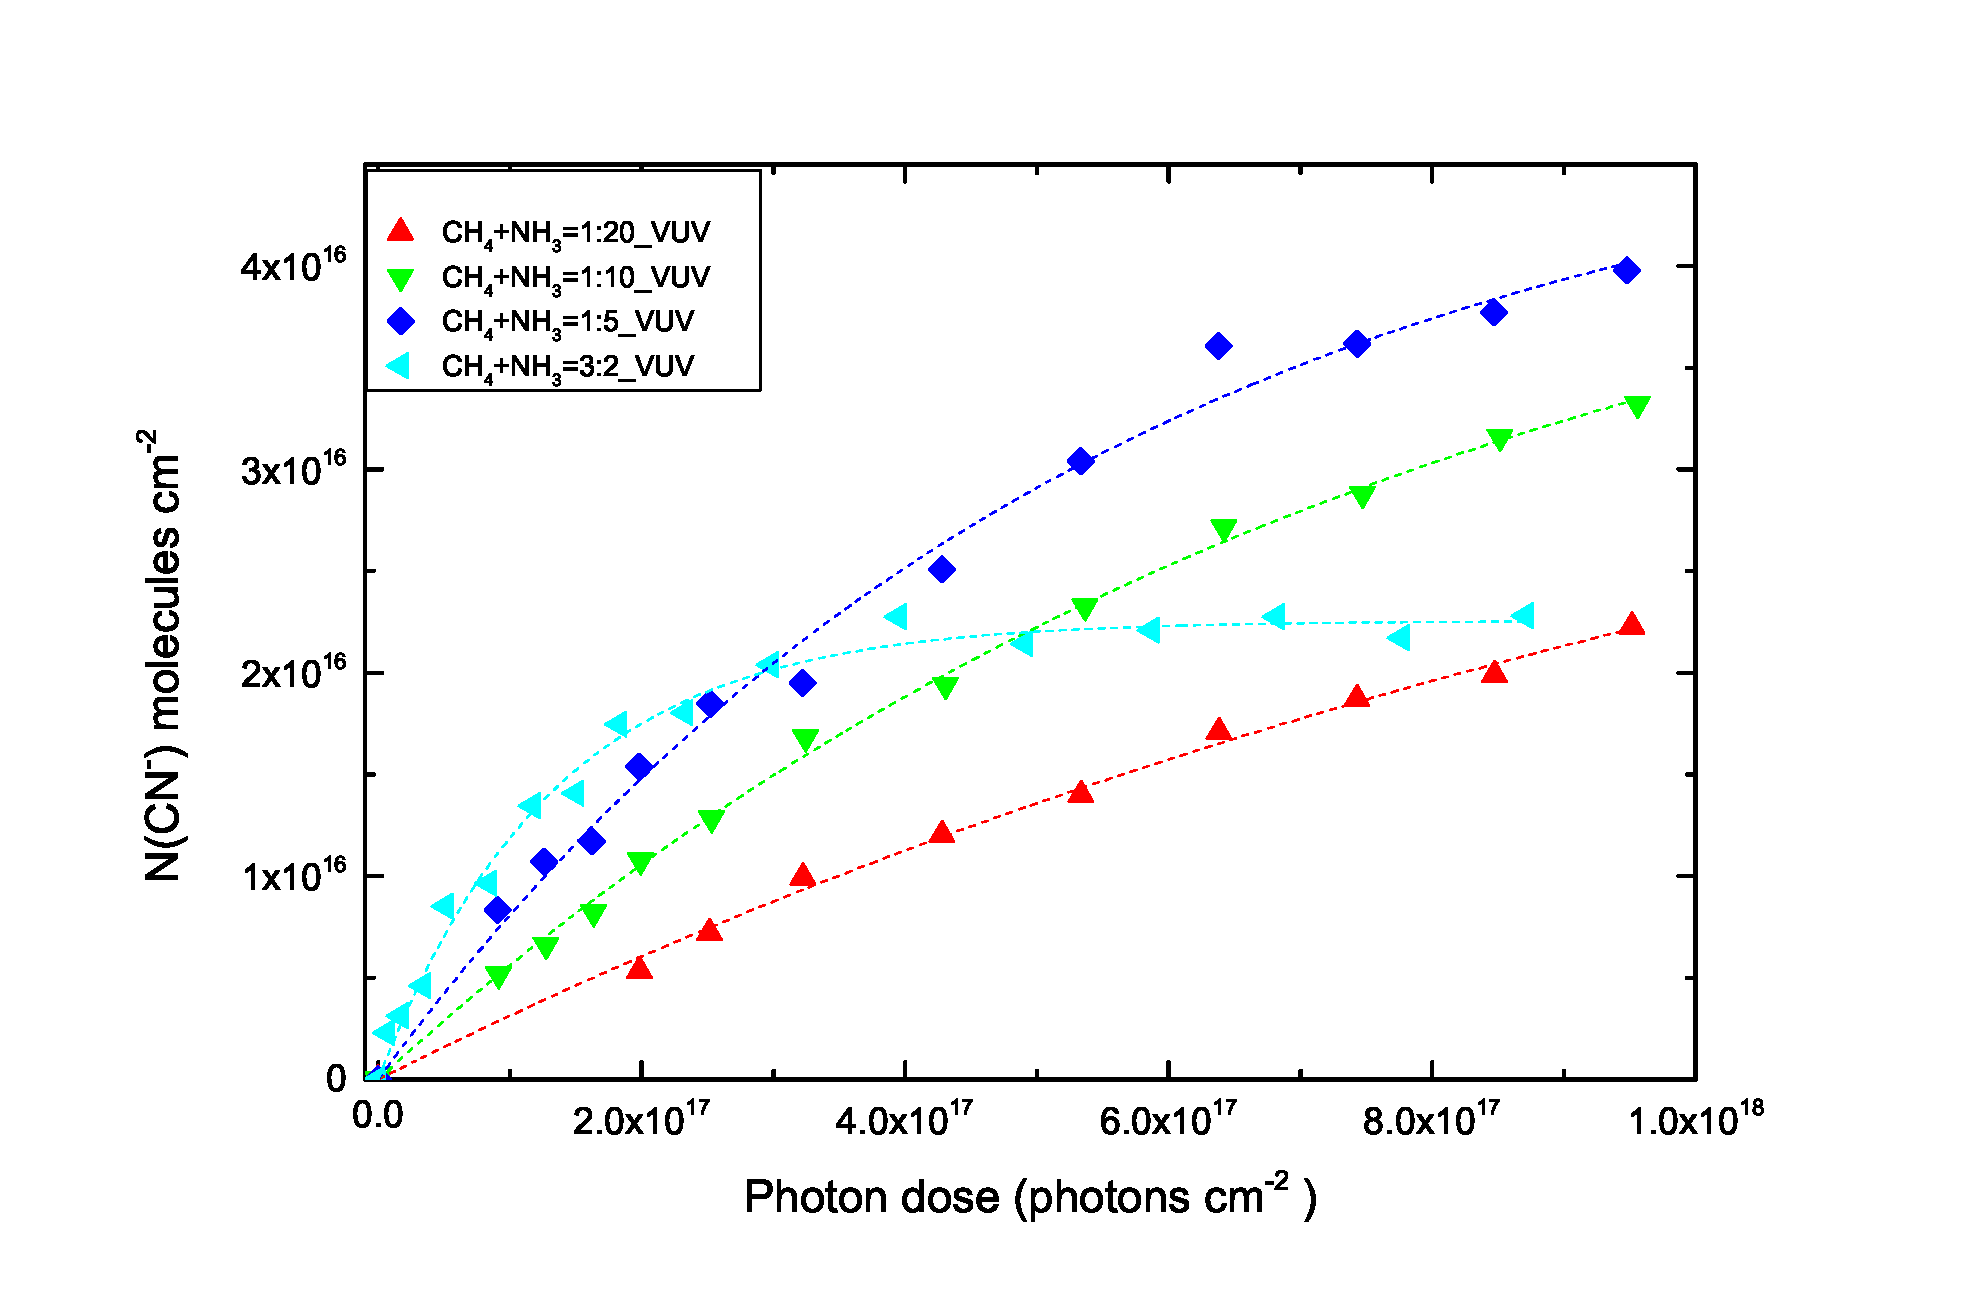
\includegraphics[width=\textwidth]{figures/chapter3/Overall_CN_rate.eps}
\caption{The column density of CN$^-$ accumulated when different configurations of CH$_4$ + NH$_3$ ice mixtures are irradiated by VUV photons provided by MDHL. The dotted lines are fits of column densities by equation \ref{eq:rate7}.}
\label{fig:CNrate}
\end{figure}

\begin{table}[htbp]
\caption{The fitting results of CN$^-$ by equation \ref{eq:rate7}}
\label{tab:CNrate}
\begin{tabular}{cccc}
\hline
\hline
Ratio of CH$_4$+NH$_3$ & A (x10$^{16}$ molecules cm$^{-2}$) & k$_1$ (x10$^{-18}$ photon$^{-1}$) & k$_2$ (photon$^{-1}$)\\
\hline
1:20 & 4.75 $\pm$ 0.40 & 0.70 $\pm$ 0.09 & >1 \\
1:10 & 4.51 $\pm$ 0.18 & 1.33 $\pm$ 0.13 & >1 \\
1:5 & 4.61 $\pm$ 0.18 & 1.93 $\pm$ 0.19 & >1 \\
3:2 & 2.24 $\pm$ 0.03 & 8.21 $\pm$ 0.70 & >1 \\
\hline
\end{tabular}\\
A represents the amount of CN$^-$ we may obtain when irradiated the ice for infinitely long.\
\end{table}

\section{The Concentration Effect in formation of Cyanide ions and Ethane}

\subsection{Cyanide ion}

From table \ref{tab:CNrate}, we may observe that the rate k$_1$ is nearly proportional to the concentration of CH$_4$.  As CH$_4$ to NH$_3$ ratio increases, more CH$_4$ are involved in CH$_3$ radical formation, thus there are more CH$_3$ radicals to produce CH$_3$NH$_2$ intermediates.

In CH$_4$ to NH$_3$ =3:2 ice mixtures, A is about half of that of the other ratios. The reduction is mainly because NH$_2$ (forming CH$_3$NH$_2$) has a competing relationship with CH$_2$, CH$_3$ and C$_2$H$_4$ radicals (forming C$_2$H$_6$ and C$_3$H$_8$). This competition supresses the production of intermediate CH$_3$NH$_2$, thus the formation of CN$^-$. Therefore, the yield of CN$^-$ is the least in CH$_4$ to NH$_3$ ice mixture with ratio 3:2 while the yield of C$_2$H$_6$ is the greatest in the mixture with the same ratio(table \ref{tab:CNrate}), (table \ref{tab:fittingC2H6})\\

Considering the normalized CN$^-$ with respect to the initial CH$_4$(figure \ref{fig:CN_CH4}), the formation of CN$^-$ is more efficient in low CH$_4$ concentration ice mixtures. At low CH$_4$ concentration, there are excess NH$_3$ which can aggregate mobile CH$_3$ radicals, preventing meeting another CH$_3$ radical or C$_2$H$_4$. Therefore the production of C$_2$H$_6$ is greatly suppressed and more CN$^-$ will be produced.

\begin{figure}
\centering
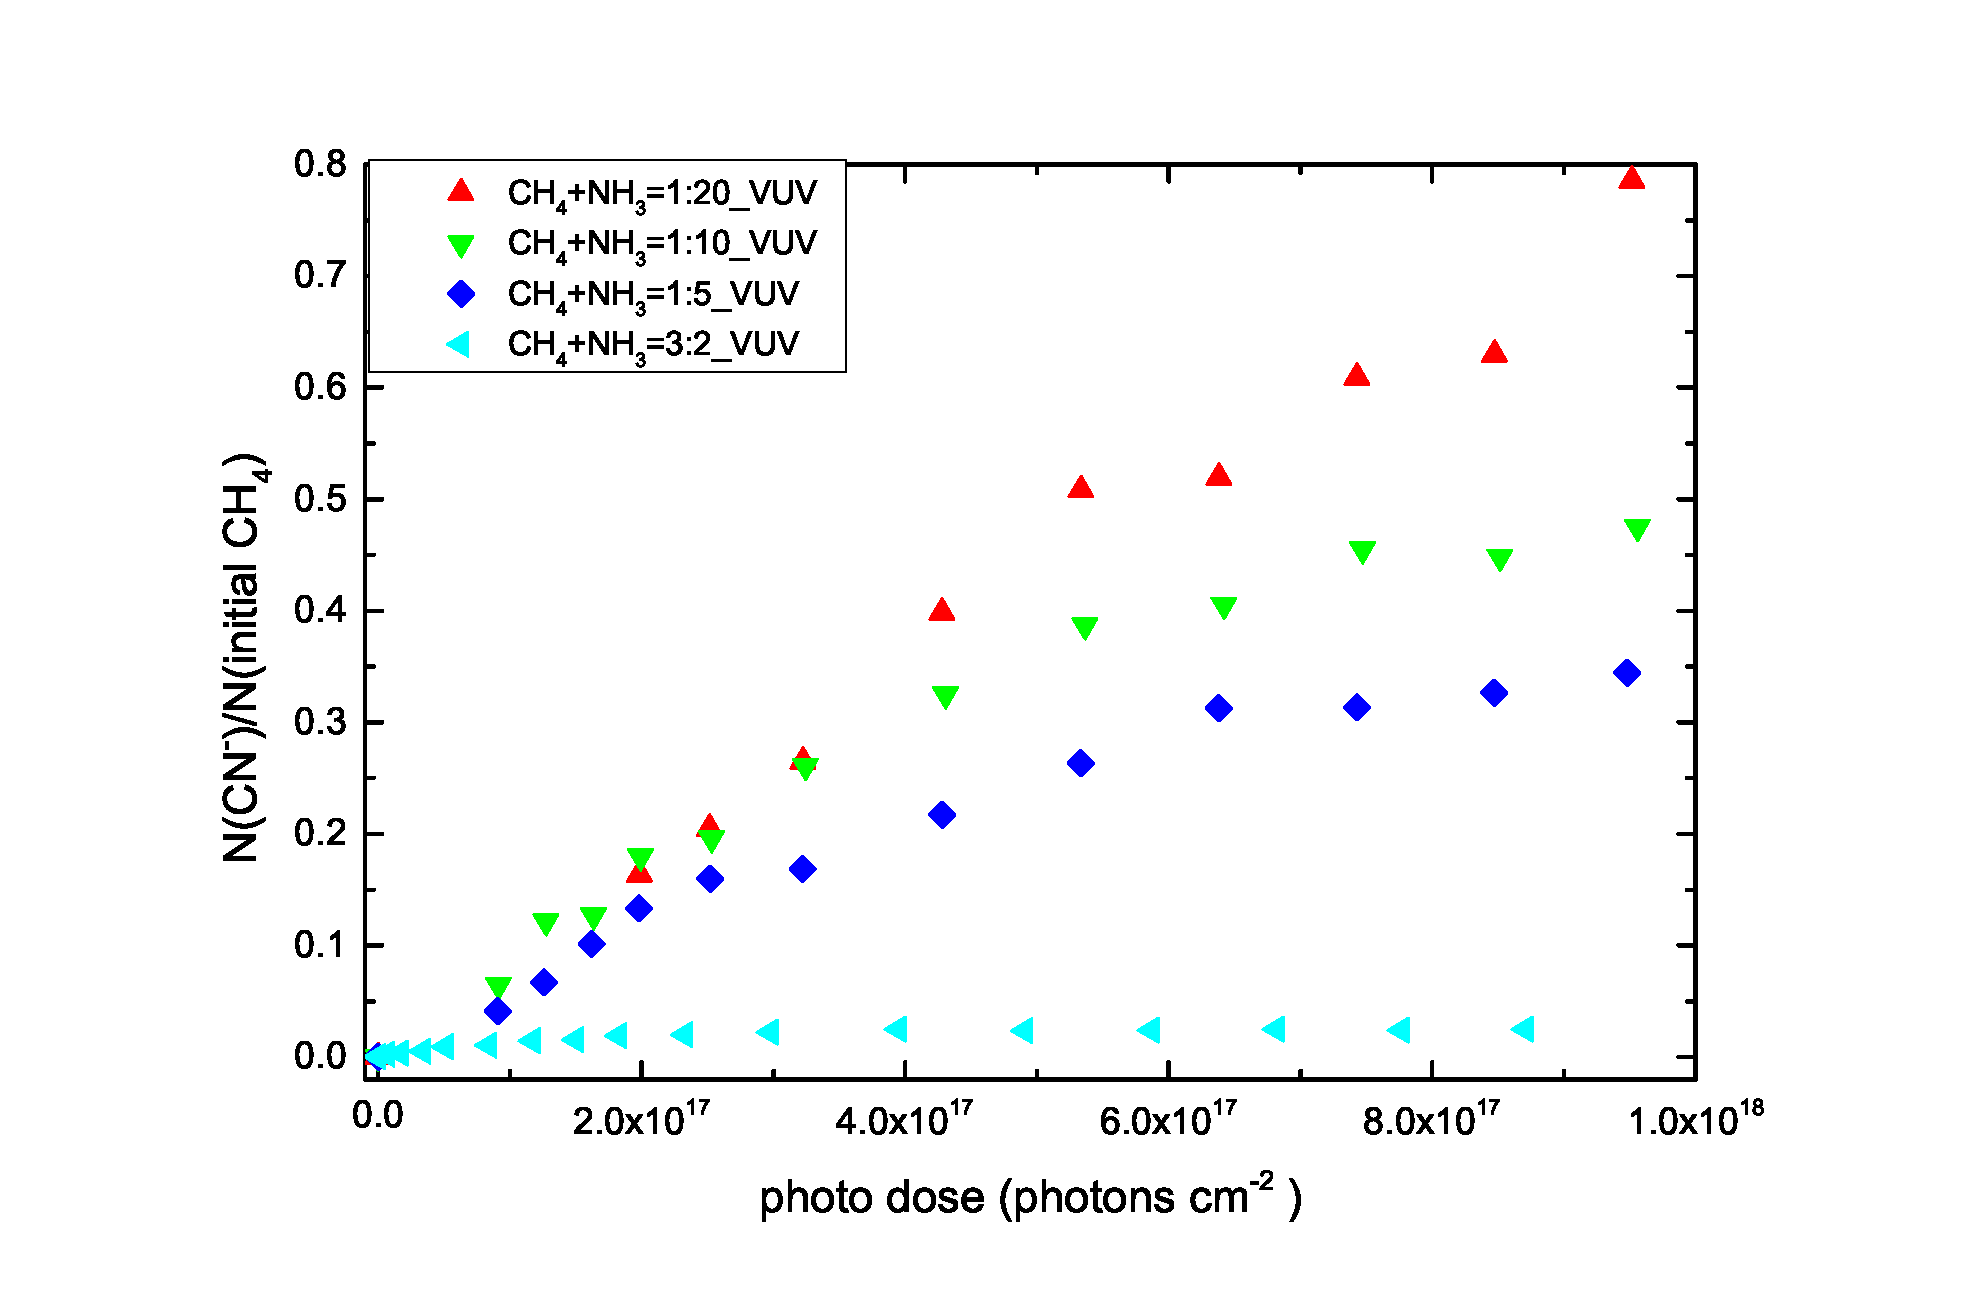
\includegraphics[width=\textwidth]{figures/chapter3/CN_CH4.eps}
\caption{The column density of CN$^-$ divided by initial CH$_4$ accumulated when different configurations of CH$_4$ + NH$_3$ ice mixtures are irradiated by VUV photons provided by MDHL.}
\label{fig:CN_CH4}
\end{figure}

\subsection{Ethane}


\begin{figure}
\centering
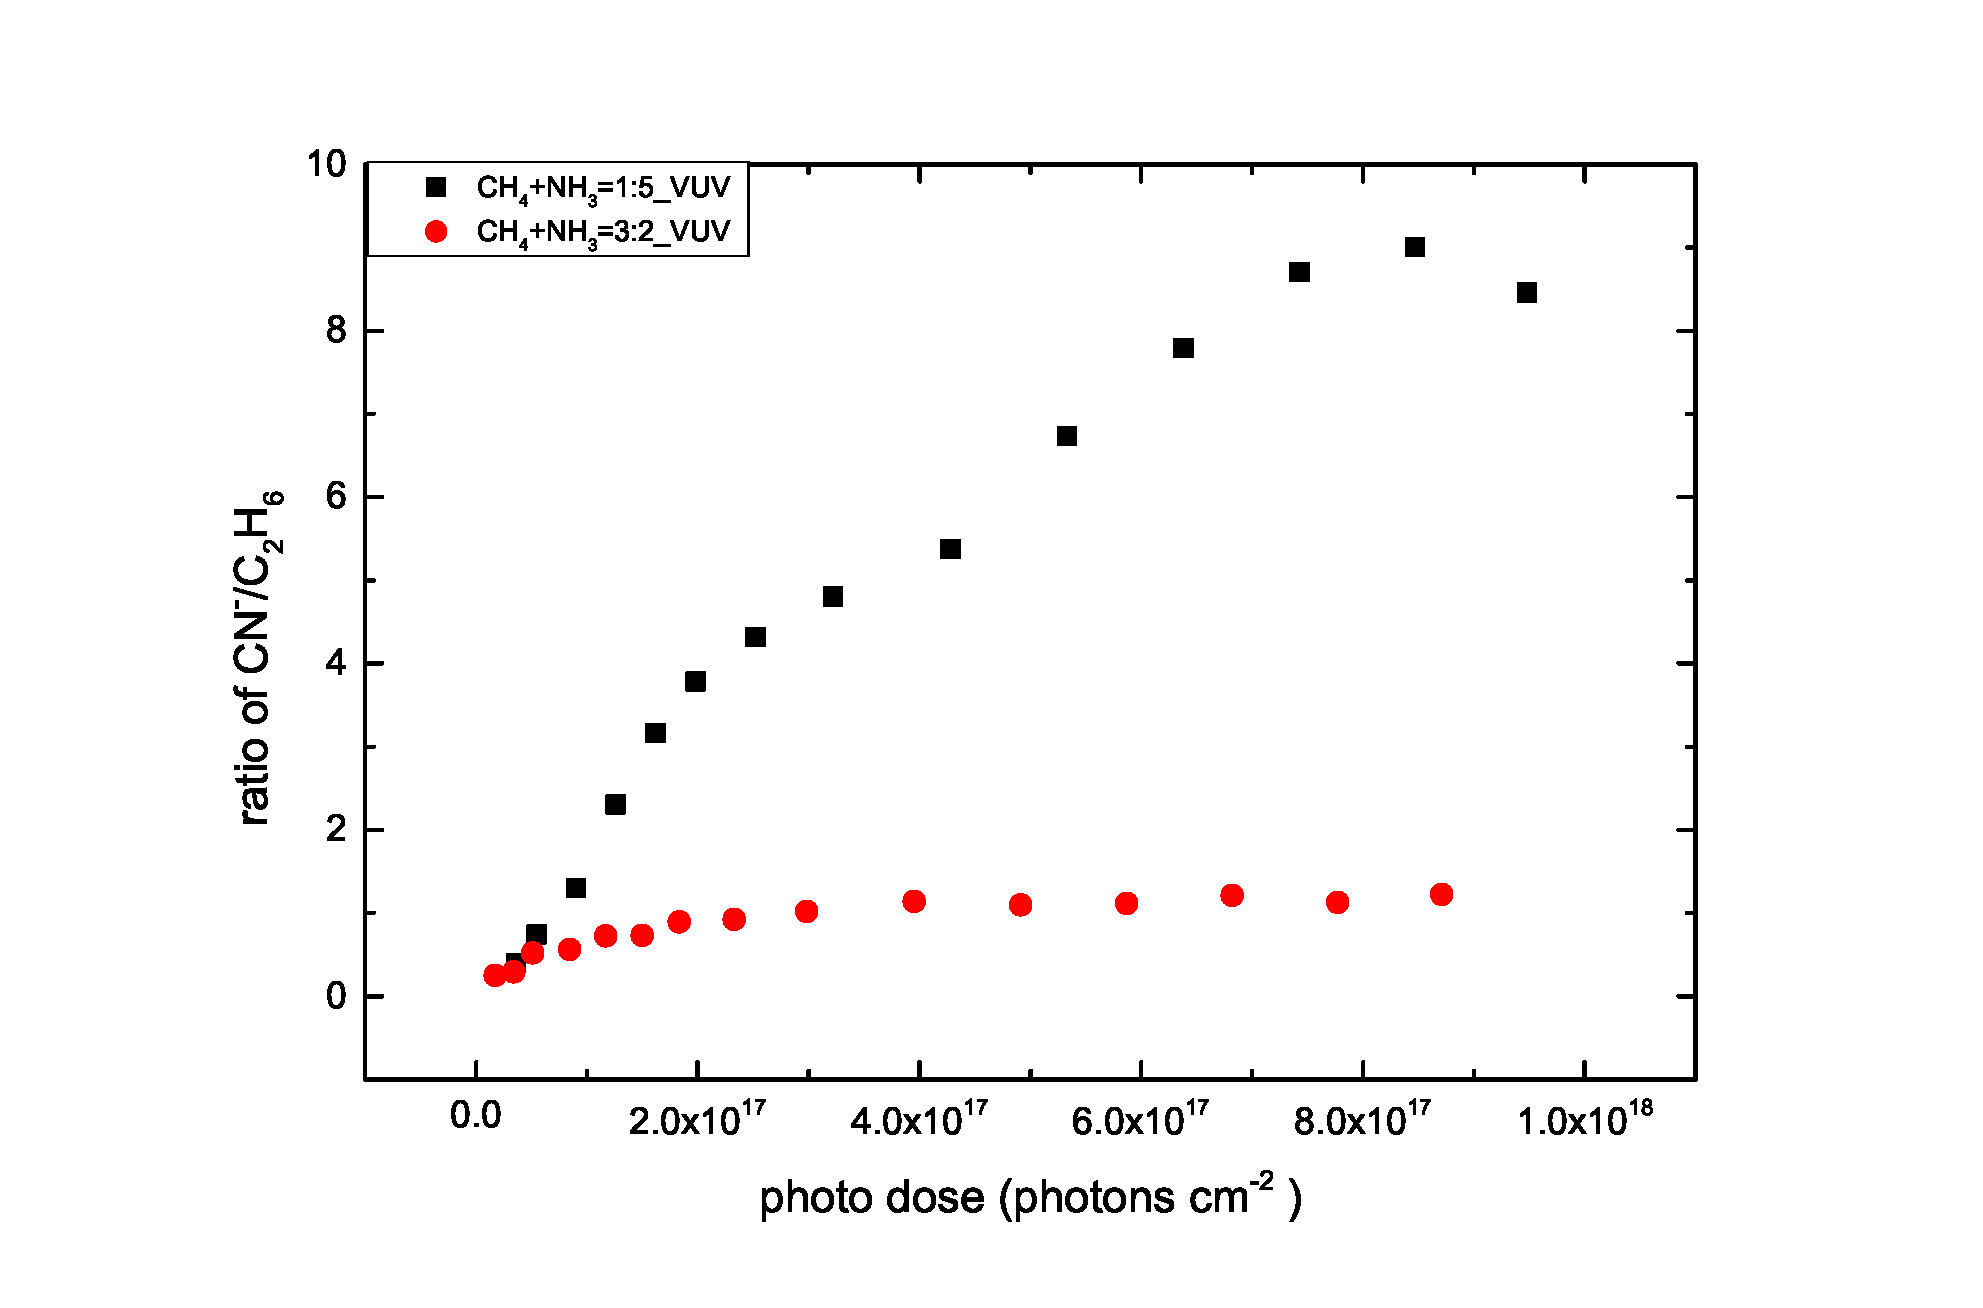
\includegraphics[width=\textwidth]{figures/chapter3/CN_C2H6.eps}
\caption{The column density of CN$^-$ divided by C$_2$H$_6$ accumulated when different configurations of CH$_4$ + NH$_3$ ice mixtures are irradiated by VUV photons provided by MDHL.}
\label{fig:C2H6_CN}
\end{figure}

Considering the case of ratio of CN$^-$ divided by C$_2$H$_6$, the formation of CN$^-$ in ice mixtures with diluted CH$_4$ has more CN$^-$ formed than C$_2$H$_6$. It is because ice mixtures with with higher concentrations in CH$_4$ is more effective for one CH$_3$ radical to combine with another CH$_3$ radical. On the contrast, CH$_3$ radicals formed in the ice mixtures with diluted CH$_4$ concentrations are aggregated by NH$_3$. Therefore, CN$^-$ is less efficient to form in ice mixtures with excess NH$_3$.

\subsection{Propane}

\begin{figure}
\centering
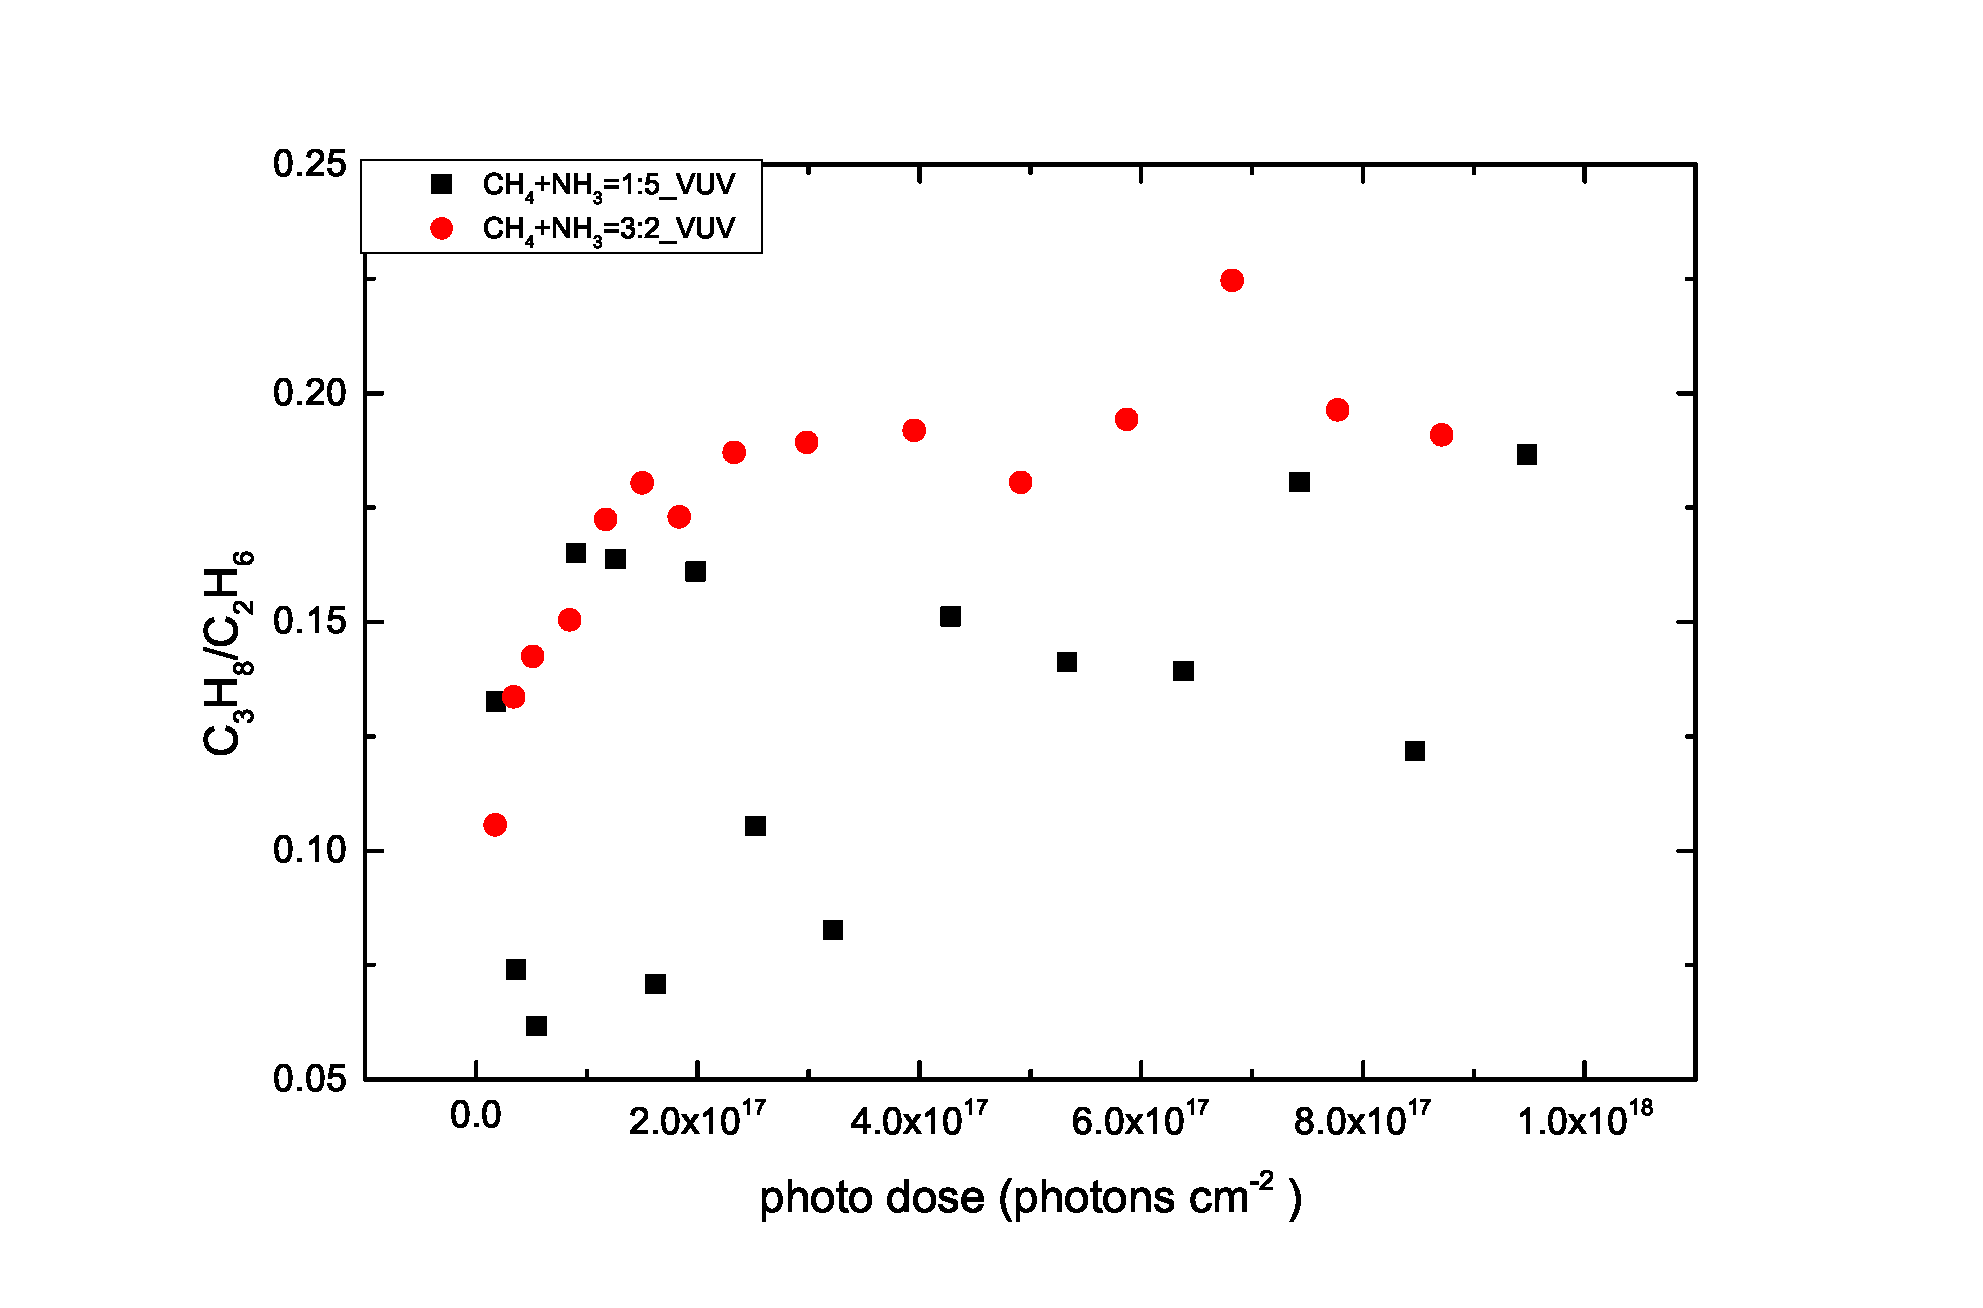
\includegraphics[width=\textwidth]{figures/chapter3/Lab_C3H8_C2H6.eps}
\caption{The column density of C$_3$H$_8$ divided by C$_2$H$_6$ accumulated when different configurations of CH$_4$ + NH$_3$ ice mixtures are irradiated by VUV photons provided by MDHL.}
\label{fig:C2H6_C3H8}
\end{figure}

C$_3$H$_8$ forms based on to the C$_2$H$_6$ \ref{fig:C2H6_C3H8} is the plot with column densities of C$_2$H$_6$ divided by C$_3$H$_8$. We may see that the ratio in CH$_4$+NH$_3$ =1:5 experiment is around 6 where CH$_4$+NH$_3$ =3:2 is around 3. This shows that the amount of C$_3$H$_8$ in CH$_4$+NH$_3$ =3:2 experiment is higher. It is rather difficult for C$_3$H$_8$ to form in CH$_4$+NH$_3$ = 1:5 experiments because NH$_3$ aggregate them. The formation of C$_3$H$_8$ in CH$_4$+NH$_3$ =1:5 and 3:2 experiments has given a reasonable explanation about why C$_2$H$_6$ formation is most efficient in CH$_4$+NH$_3$ =1:10 experiments.



\section{Photon Energy Effect - EUV and VUV} %EUV & VUV

According to Blanksby and Ellison (2003) \cite{blanksby2003bond}, the dissociation energy for CH$_4$, becoming CH$_3$, CH$_2$, CH and C are 4.55, 4.79, 4.39 and 3.51 eV respectively at 298 K. Whereas dissociation energy for NH$_3$, becoming NH$_2$ is 4.67 eV at 298 K.

Considering our MDHL with average energy of 9.27 eV, all of the above fragments may exist either in the form of radicals or combine with other radicals to form heavier molecules in our ice mixtures. Although increasing the photon energy does not create new fragmentation pathway, the choice of fragmentation pathways depends on photon energy.

Several gaseous state measurements also support this statement. First, Gans et al. (2011) \cite{gans2011photolysis} changed VUV photon wavelengths from 121.6 nm (10. 2eV) to 118.2 nm (10.4eV) to dissociate the CH$_4$ molecules and ionize the fragments with the corresponding photon energy. Changing the output of the pulsed laser from 121.6 to 118.1 nm significantly changed the ratio of CH$_3^+$ and CH$_2^+$, produced from fragmentation, from 1: 1 to 1:2. This slight change of photon energy, from 10.2 eV to 10.4 eV has a significant change in the ratio between different pathways.

Second, an EUV fragmentation experiment done by Tsai et al. \cite{tsai1980mass} used 30.4 nm to photo-dissociate CH$_4$ and tested it by time$-$of$-$flight mass spectrometer yields CH$_3^+$: CH$_2^+$: CH$^+$: C$^+$ = 1 :0.32: 0.118: 0.0237 (Tsai 1980). Consider the ratios of CH$_3$ to CH$_2$ radicals, it is around 3 to 1, which is in contrast to the experiment results of Gans et al. (2011)\cite{gans2011photolysis}. Although both of them are gaseous state experimental results, it is uncertain whether increasing photon energy can produce more CH$_2$ radicals in ice mixtues.

Thirdly, a group varies ratios of CH$_4$ + NH$_3$ mixtures and irradiate with far UV irradiation at 134 nm \cite{bossard1980far}. However, this group only used gas chromatography to analyse the final products and their reaction is carried in gas phase in room temperature. We aware that the VUV absorption spectra of CH$_4$ in solid phases is different from gaseous phases \cite{cruz2014vacuum}, so the exact photo dissociation fragmentation ratios by EUV nor VUV irradiations in astronomical environments are still unknown. It is worthwhile for us to perform the experiment by EUV irradiation to see if  EUV irradiation can generate any new products on the surface of Charon, or any difference in yield. Despite the photon energy of our MDHL is enough to dissociate both the CH$_4$ and NH$_3$ molecules, we further increase photon energy to He II 30.4 nm to examine the differences in photo-products. 

\begin{figure}
\centering
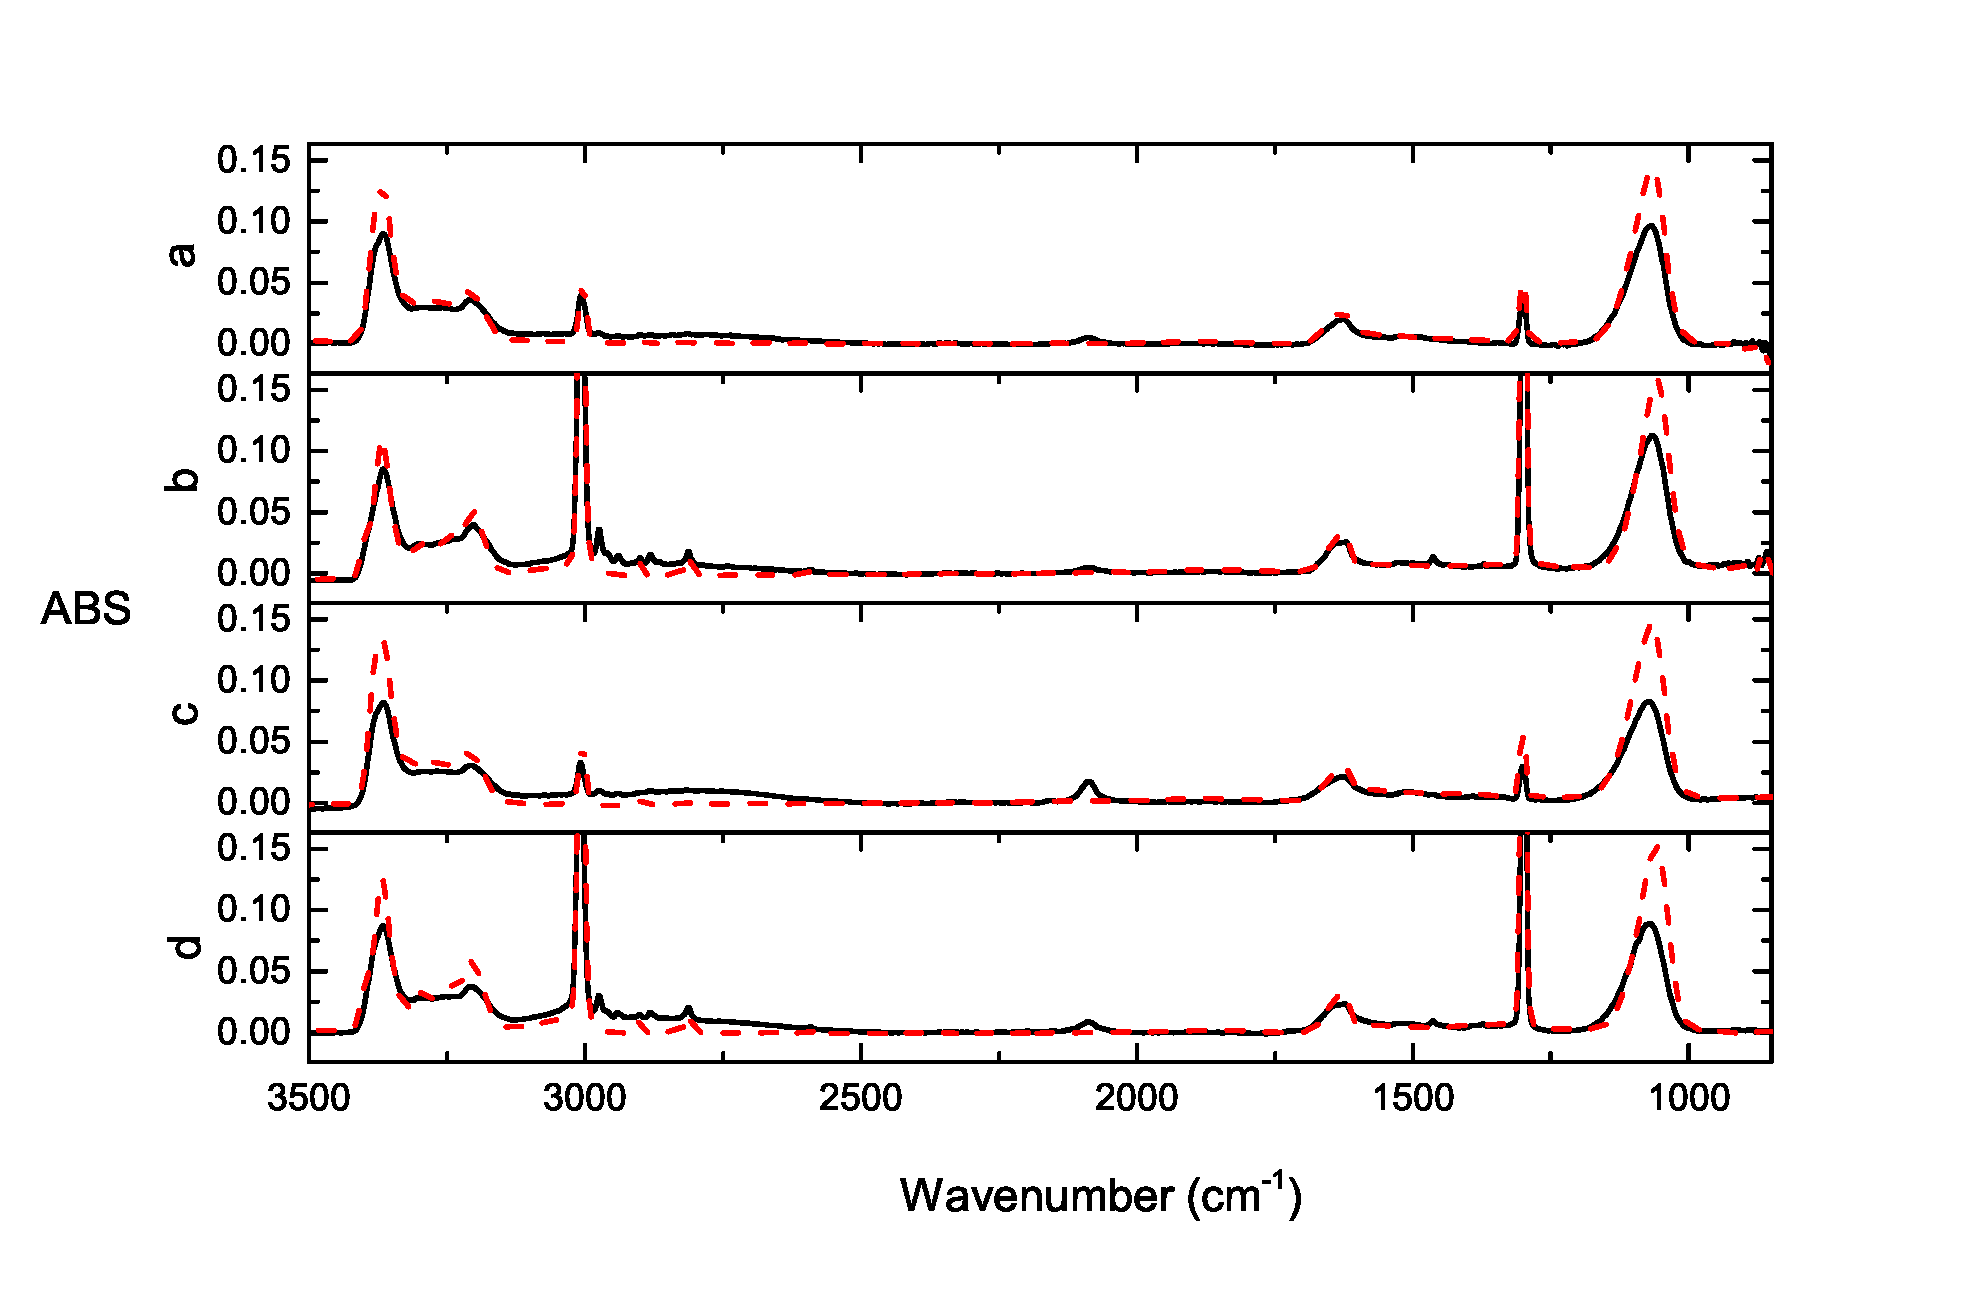
\includegraphics[width=\textwidth]{figures/chapter3/NSRRC_MDHL_IR.eps}
\caption{The the infra-red spectrum of CH$_4$ + NH$_3$ ice mixtures before irradiation (dashed) and VUV and EUV (solid) irradiated ice mixtures provided by MDHL. (a) and (b) are EUV irradiated CH$_4$+NH$_3$ = 1:5 and 3:2 ice mixtures respectively, and (c) and (d) are VUV irradiated CH$_4$+NH$_3$ = 1:5 and 3:2 ice mixtures respectively.}
\label{fig:NSRRC_MDHL_IR}
\end{figure}

Table \ref{tab:WavenumberNSRRC} shows the identified peaks of CH$_4$+NH$_3$ ice mixtures irradiated by VUV and EUV (30.4 nm) irradiated in IR spectra (figure \ref{fig:NSRRC_MDHL_IR}).

\begin{table}[htbp]
\caption{The peak positions of identified substances after VUV and EUV irradiations in different configurations of ice mixtures.}
\label{tab:WavenumberNSRRC}
\begin{tabular}{ccccccc}
\hline
\hline
\multicolumn{2}{c}{Literture assignments} & \multicolumn{2}{c}{CH$_4$+NH$_3$ ratio (MDHL)} & \multicolumn{2}{c}{CH$_4$+NH$_3$ ratio (30.4 nm)} \\
\hline
Wavenumber & Carrier  & 1:5 & 3:2 & 1:5 & 3:2 & Ref. \\
(cm$^{-1}$) &   & (cm$^{-1}$) & (cm$^{-1}$) & (cm$^{-1}$) & (cm$^{-1}$) &\\
\hline
3375 & $\nu_3$ (NH$_3$) & 3366 & 3367 & 3368 & 3368 & 1 \\
3290 & $2\nu_4$ (NH$_3$) & - & - & - & - & 1 \\
3210 & $\nu_1$ (NH$_3$) & 3207 & 3205 & 3209 & 3205 &1 \\
3011 & $\nu_3$ (CH$_4$) & - & - & - & - & 2 \\
2972 & $\nu_{10}$ (C$_2$H$_6$) & 2975 & 2975 2977 & 2976 & & 3 \\
2960 & C$_3$H$_8$ & - & 2960 & - & 2960 & 7 \\
2941 & $\nu_8+\nu_11$ (C$_2$H$_6$) & 2940 & 2940 & - & 2942 & 3 \\
2904 & $\nu_1$ (CH$_4$) & 2901 & 2901 & 2901 & 2901 & 5 \\
2879 & $\nu_5$ (C$_2$H$_6$) & 2882 & 2882 & - & 2884&  3 \\
2814 & $\nu_2+\nu_4$ (CH$_4$) & - & 2815 & - & 2813 & 5 \\
2083 & $\nu$ (CN$^-$) & 2088  & 2088 & 2090 & 2089 & 2 \\
1625 & $\nu_4$ (NH$_3$) & 1625 & 1631 & 1627 & 1631 & 1 \\
1514 & $\delta$ (NH$_2$) & 1509 & 1511 & 1509 & 1511 & 6 \\
1465-1440 & deform CH$_2$ scissor & 1461 & 1463 & - & 1465 & 3,4 \\
1390-1370 & CH$_3$ sym deform & 1394 & 1372 & - & 1372 & 4 \\
1298 & $\nu_4$ (CH$_4$) & 1301 & 1299 & 1303 & 1301 & 2 \\
1075 & $\nu_2$ (NH$_3$) & 1073 & 1072 & 1070 & 1068 & 1 \\
820 & $\nu_12$ (C$_2$H$_6$) & - & 820 & - & - & 3 \\
\hline
\end{tabular}\\
Reference: 1. Bossa et al. (2008) \cite{bossa2008carbamic} 2. Moore and Hudson (2003) \cite{moore2003infrared} 3. Kim et al. (2010) \cite{kim2010abiotic} 4. Socrates et al. (2001) \cite{socrates2001infrared} 5. Bennet and Kaiser (2007) \cite{bennett2007formation} 6. Zheng et al. (2008) \cite{zheng2008formation} 7. Hudson and Moore (2004) \cite{hudson2004reactions}
\end{table}


Considering the formation mechanisms of C$_2$H$_6$ and C$_3$H$_8$, equation (\ref{eq:C2H6} and \ref{eq:C3H81}), when MDHL VUV irradiation is replaced by He II 30.4 nm monochromatic light, the ratio of C$_2$H$_6$ to C$_3$H$_8$ in CH$_4$ to NH$_3$ = 3:2 ice mixtures irradiated by VUV irradiation is lower under EUV irradiation than that  under EUV provided by NSRRC (figure \ref{fig:NSRRC_Lab_C3H8_C2H6}). There are two possible explanations. First, different photon energies flavour different CH$_4$ fragmentation pathway and less C$_3$H$_8$ is produced with EUV photons. Second, the efficiency of CH$_4$ fragmentation is greatly reduced under EUV irradiation and the density of CH$_3$ radicals are much lower than that in the case of VUV irradiation provided by the MDHL. We lengthen the time of EUV irradiation on our ice mixtures until the total number of destructed CH$_4$ is similar to that in VUV irradiation experiments done with MDHL. The averages of ratios of C$_2$H$_6$:C$_3$H$_8$ of the last 7 irradiations before terminating irradiations are 3.53 in VUV and 3.66 in EUV. The result supports the latter explanation. From figure \ref{fig:normalized_reactants}, The reduction of CH$_4$ is 6.06$\pm$ times slower in EUV experiments than VUV experiments while the reduction of NH$_3$ is 3.19$\pm$0.12 times lower. Therefore, the destruction cross-section of CH$_4$ and NH$_3$ ice has a 6.06$\pm$0.07 and 3.19$\pm$0.12 times lower in 30.4 nm than in 121.6 nm.

\begin{figure}
\centering
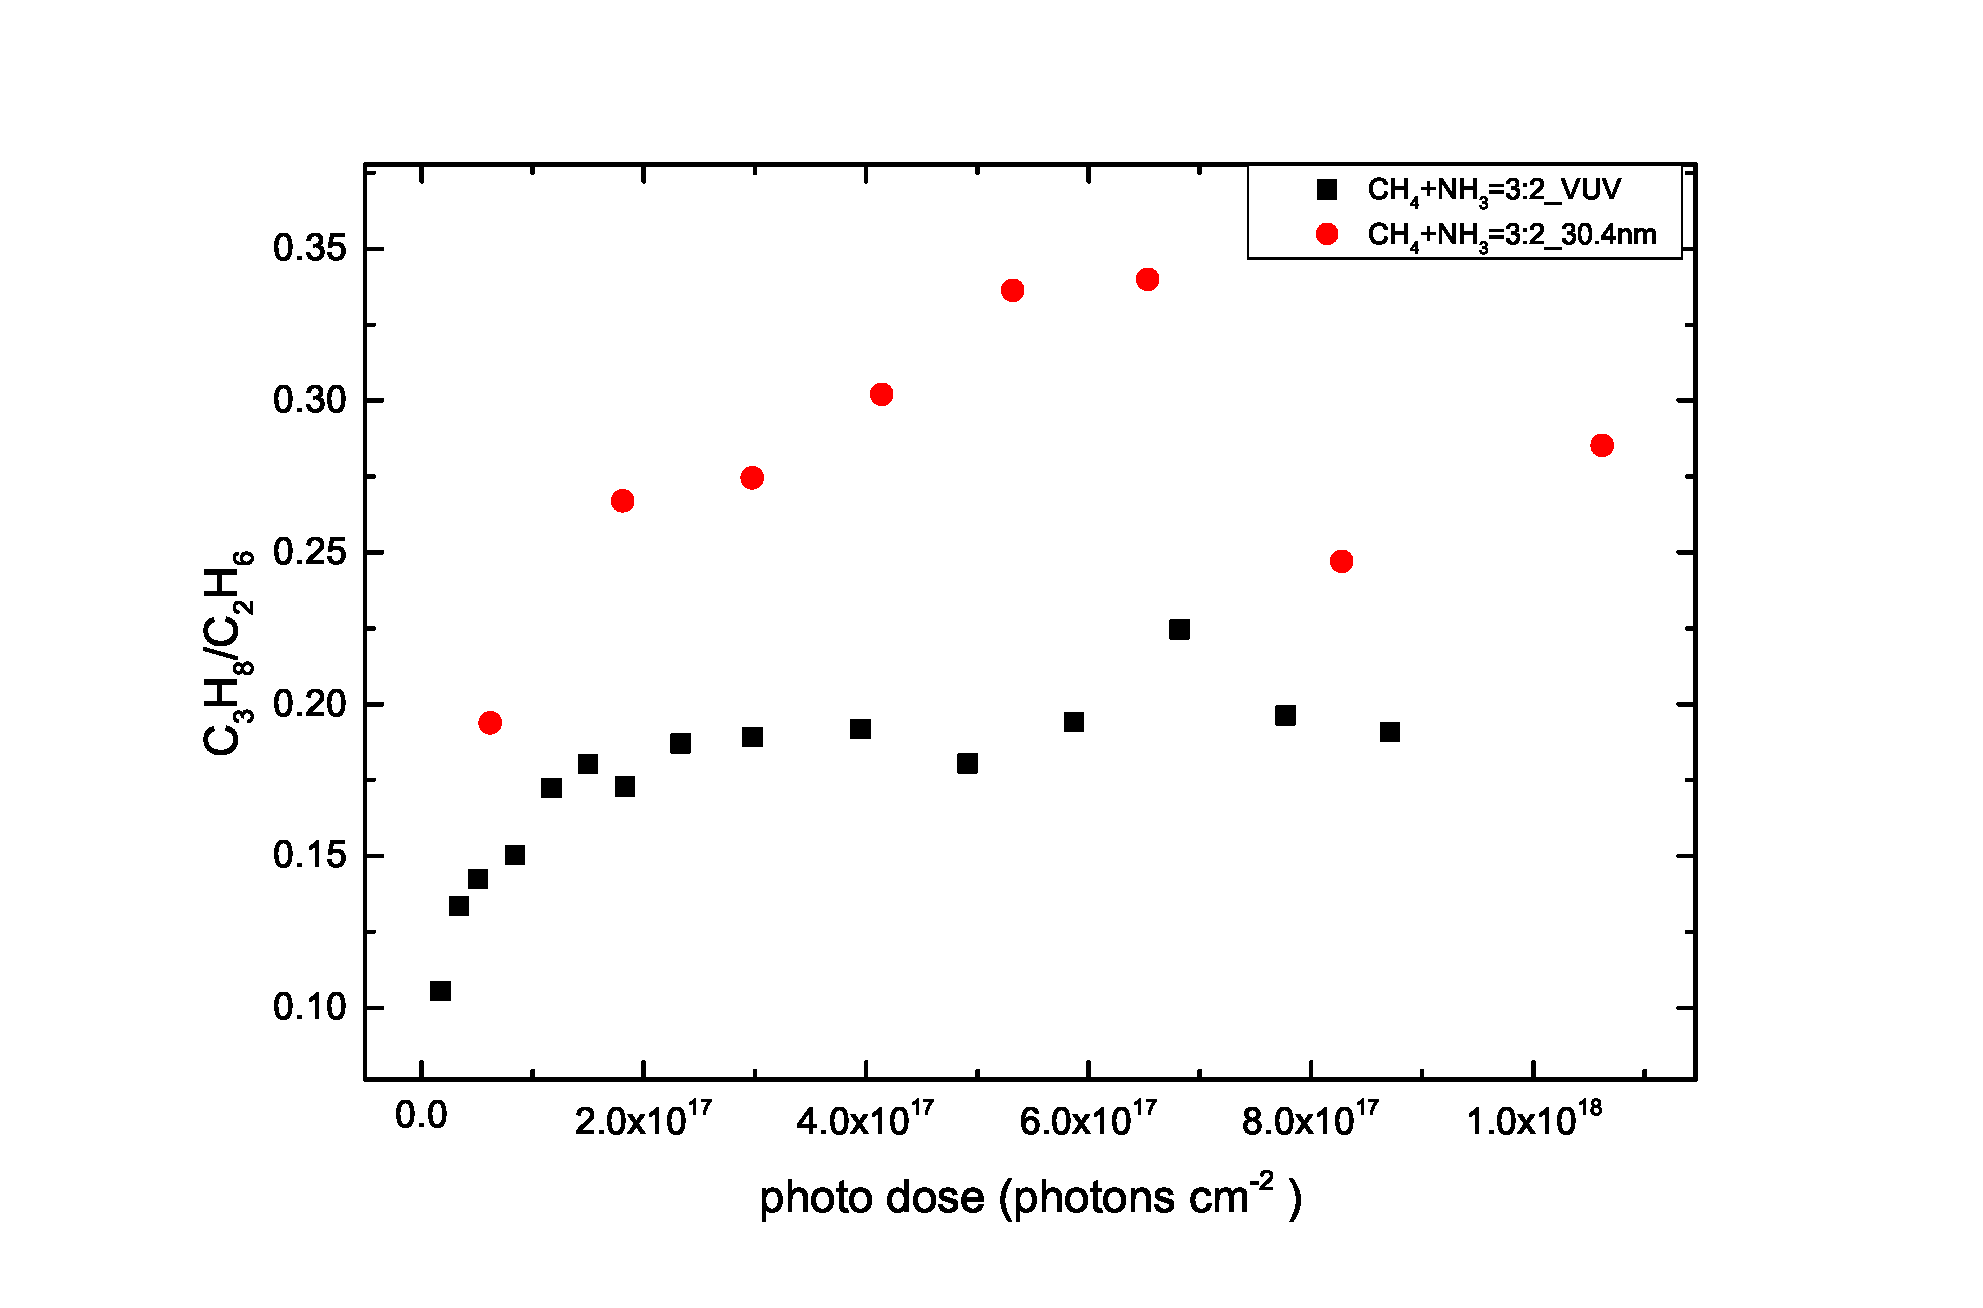
\includegraphics[width=\textwidth]{figures/chapter3/NSRRC_Lab_C3H8_C2H6.eps}
\caption{The column density of C$_3$H$_8$ divided by C$_2$H$_6$ accumulated when different configurations of CH$_4$ + NH$_3$ ice mixtures are irradiated by VUV and EUV photons}
\label{fig:NSRRC_Lab_C3H8_C2H6}
\end{figure}

Figure \ref{fig:NSRRC_Lab_C3H8_C2H6} shows the column densities of C$_2$H$_6$ divided by C$_3$H$_8$ after CH$_4$ + NH$_3$ =3:2 ice mixtures are irradiated by VUV irradiation and He II monochromatic light.

From \ref{fig:NSRRC_Lab_C3H8_C2H6}, we may observe that more C$_3$H$_8$ is produced by 30.4nm photons than by VUV photons. Recall the formation mechanism of C$_3$H$_8$ (equation \ref{eq:C3H82}), CH$_2$ and C$_2$H$_4$ radicals are esccential in producing C$_3$H$_8$. This increase production in C$_3$H$_8$ may be caused by the increase in CH$_2$ radicals during fragmentation of CH$_4$. This result is similar to the findings of Gans et al. (2011)\cite{gans2011photolysis}, the ratio of CH$_2$ radicals increases from 0.3 to 0.48 when photon energy increases from 121.6 nm to 118.2 nm in their pulsed laser experiments.


\begin{figure}
\centering
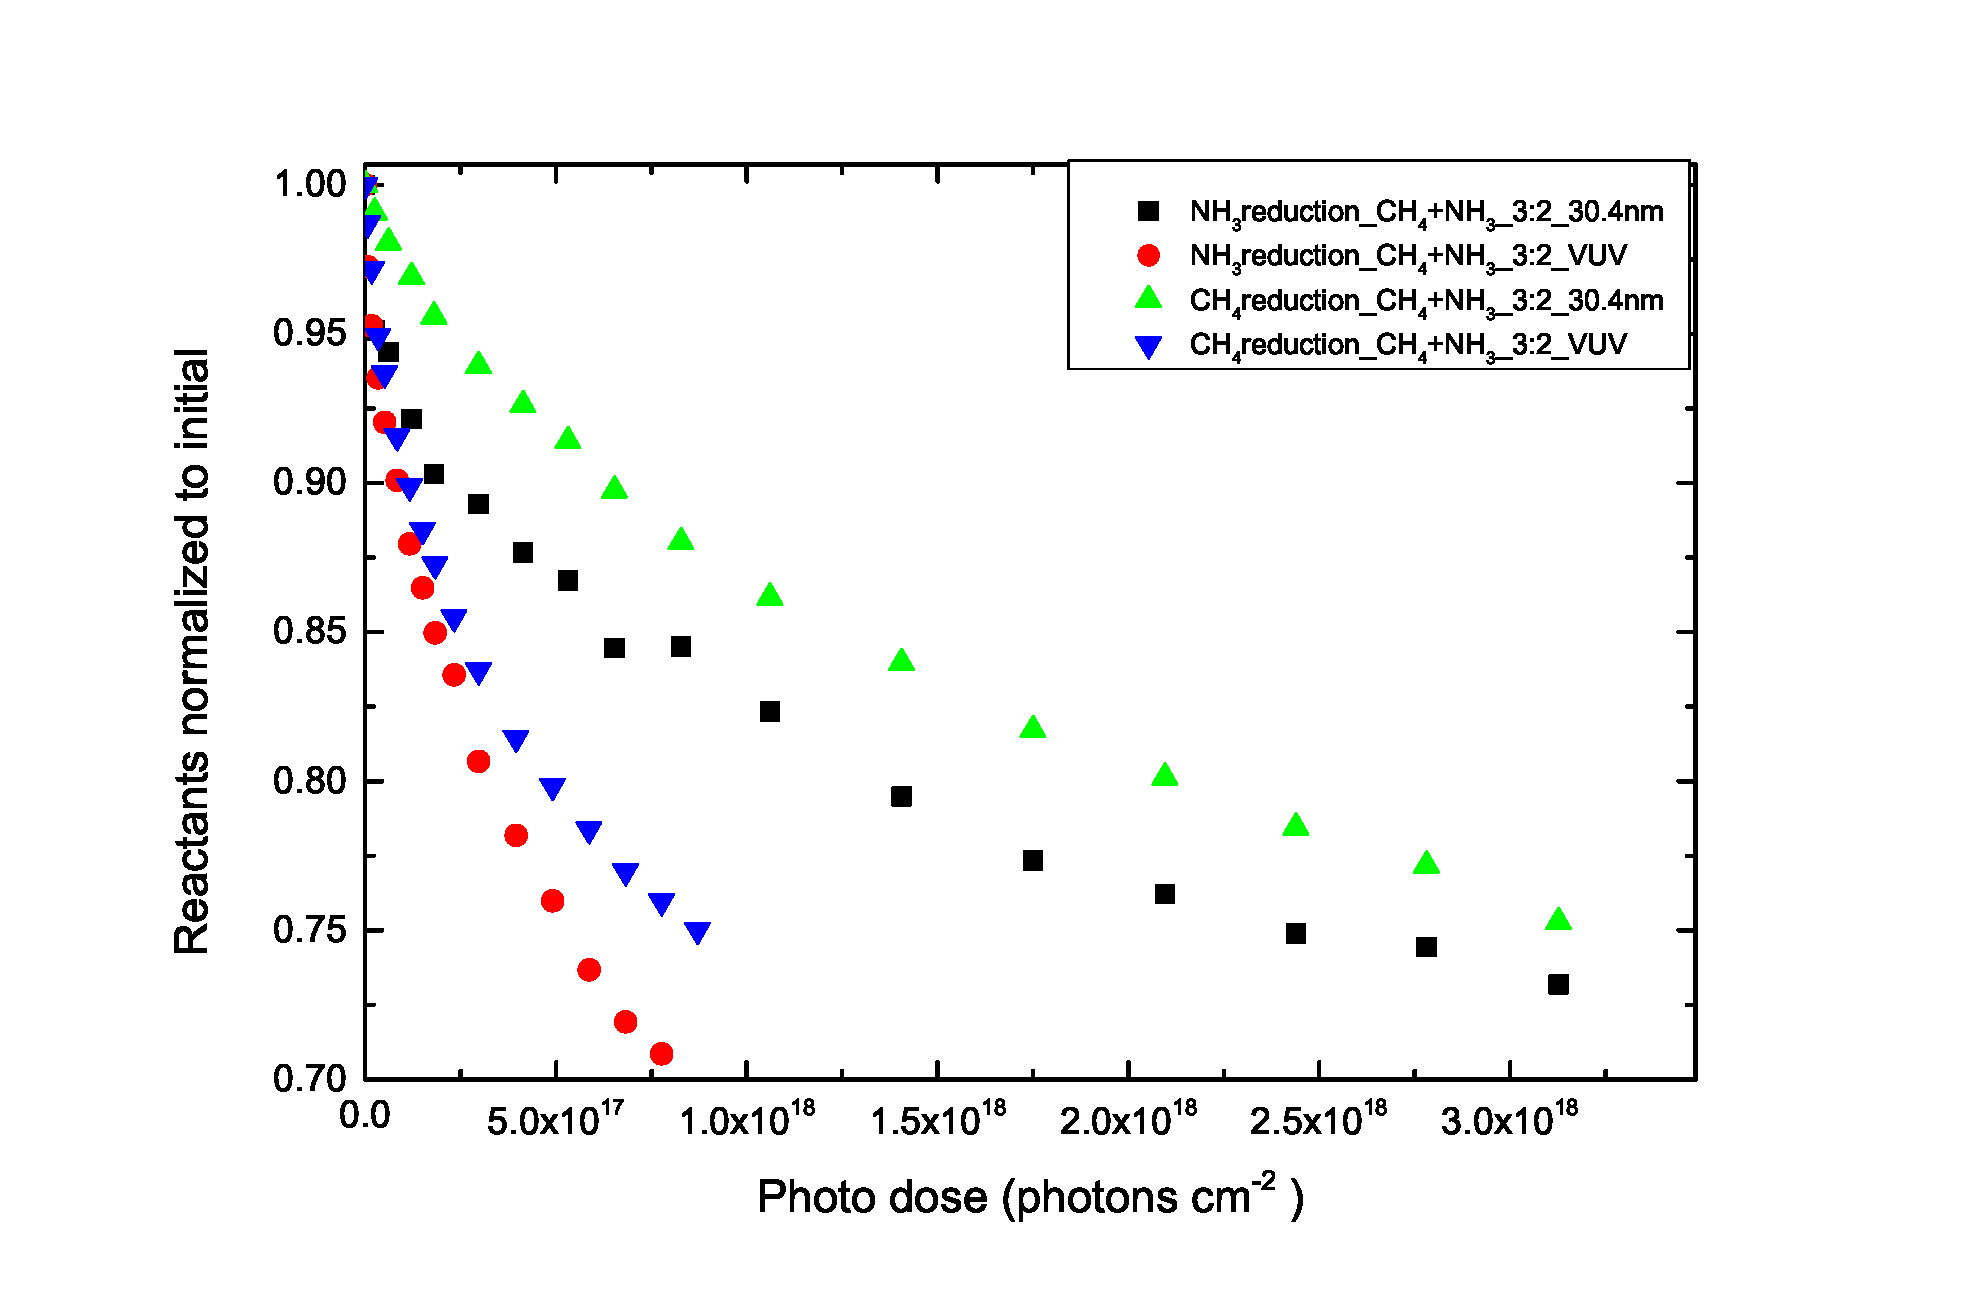
\includegraphics[width=\textwidth]{figures/chapter3/Reactants_normalized_to_initial.eps}
\caption{The normalized reduction of CH$_4$ and NH$_3$ in CH$_4$ + NH$_3$ ice mixtures irradiated by VUV and EUV photons}
\label{fig:normalized_reactants}
\end{figure}

Apart from C$_2$H$_6$ and C$_3$H$_8$, are there any difference in CN$^-$ production? Figure \ref{fig:CN_NSRRC} shows the accumulated column densities of CN$^-$ generated by irradiation of CH$_4$+NH$_3$ ice mixtures by MDHL and 30.4 nm monochromatic light. The fitting results are shown in Table 3.6. The rate constants forming CN$^-$ is 3.06 to 4.13 times larger in CH$_4$+NH$_3$ = 1:5 and 3:2 irradiated by MDHL than irradiated by 30.4 nm monochromatic light respectively. From figure \ref{fig:normalized_reactants}, the destruction cross-section of CH$_4$ and NH$_3$ are reduced by 6.06$\pm$0.07 and 3.19$\pm$0.12 times respectively. The formation rate constants of CN$^-$ is 3.06 to 4.13 times smaller than VUV irradiations (table \ref{tab:CNrate_NSRRC}. Therefore, we may conclude that the reduction in CN$^-$ formation rate by 30.4nm EUV irradiation is mainly due to the decreased NH$_3$ destruction cross-sections.

\begin{figure}
\centering
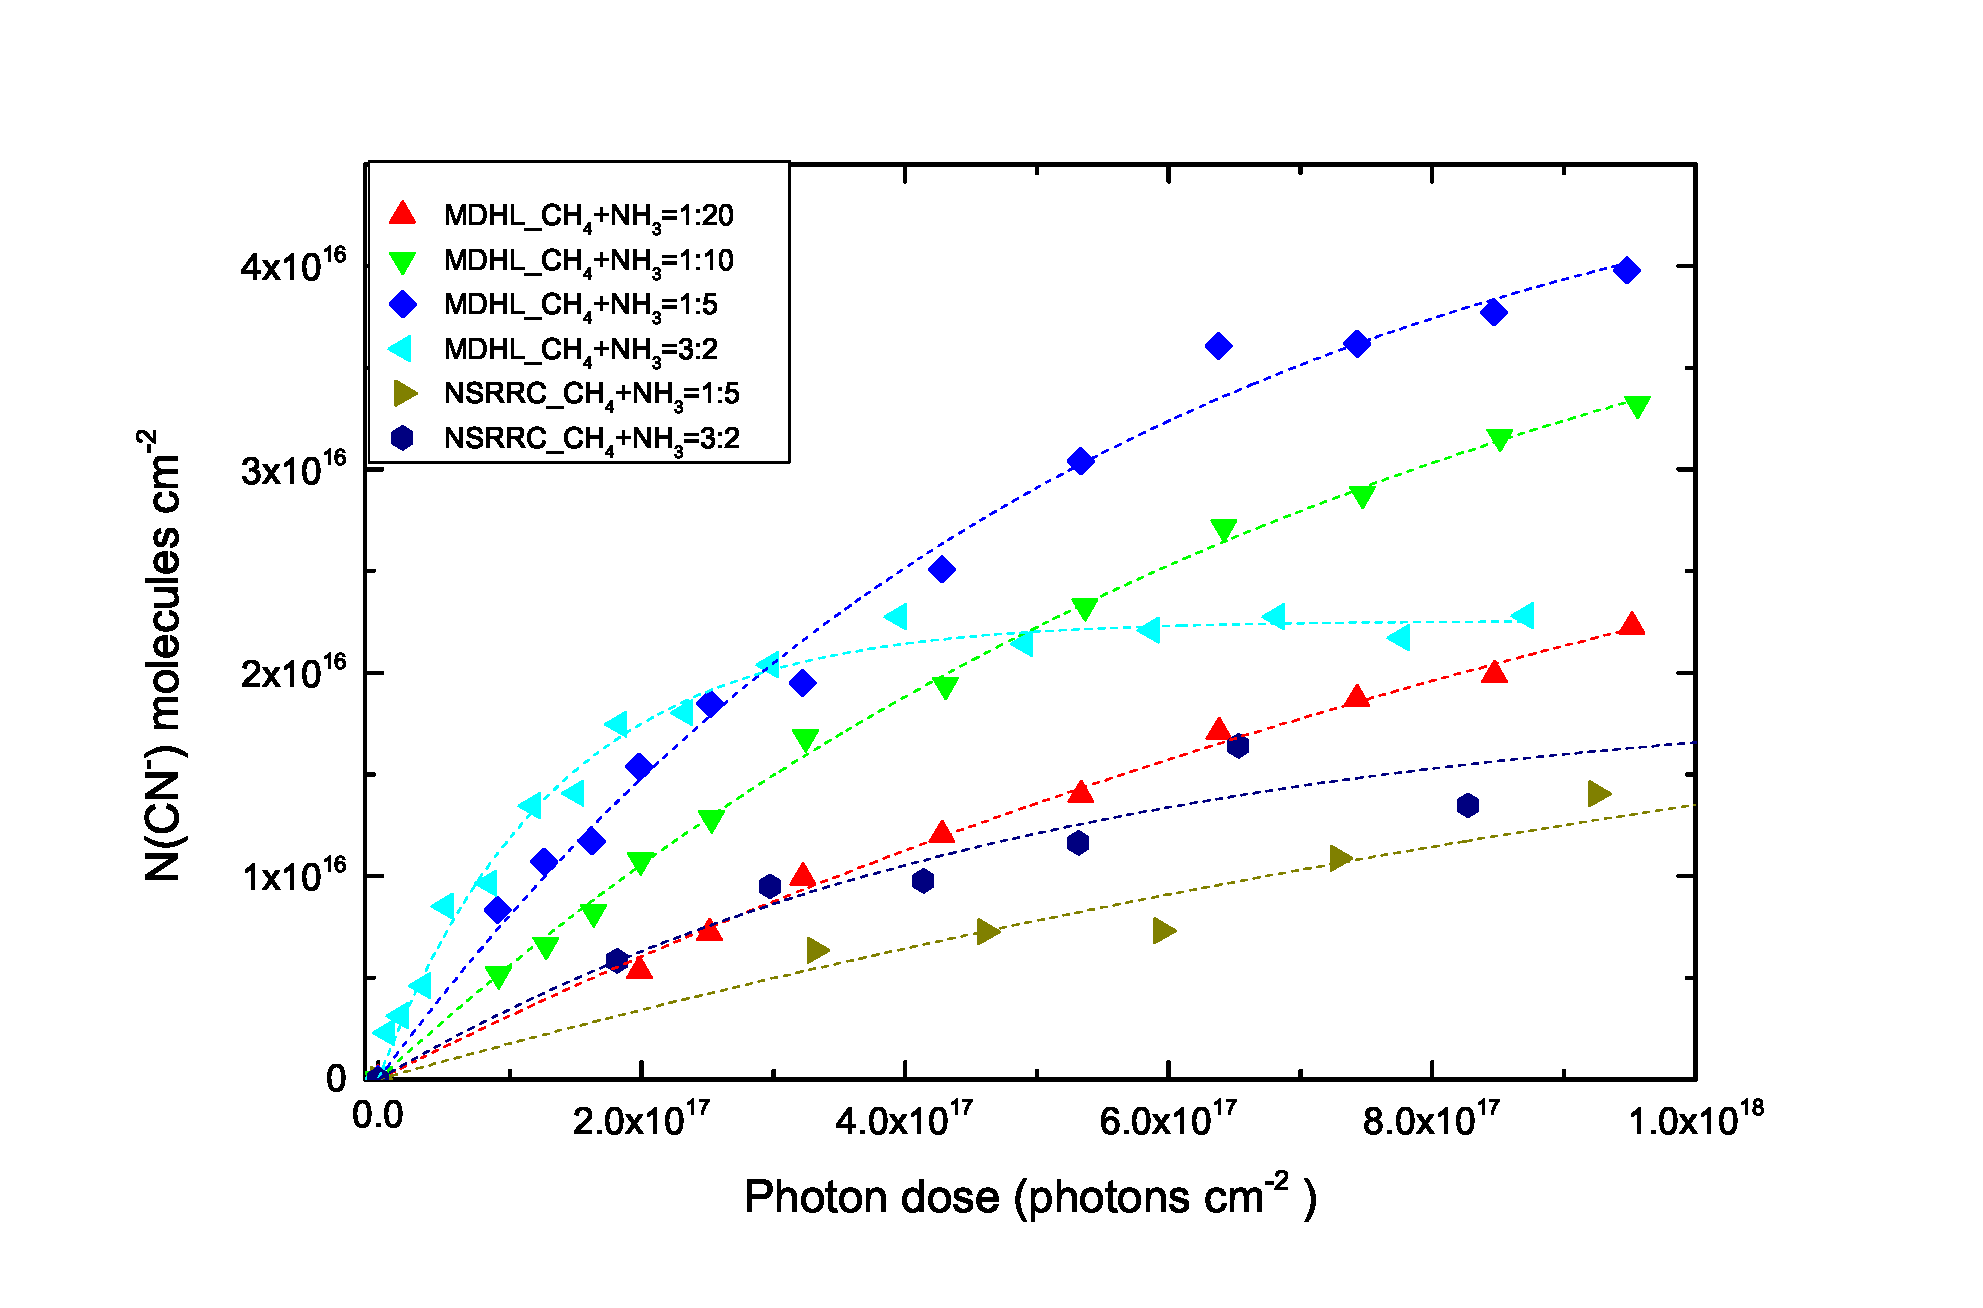
\includegraphics[width=\textwidth]{figures/chapter3/overall_CN_NSRRC.eps}
\caption{The column densities of CN$^-$ generated by irradiation of CH$_4$+NH$_3$ ice mixtures by MDHL and 30.4 nm monochromatic light.}
\label{fig:CN_NSRRC}
\end{figure}

\begin{table}[htbp]
\caption{The fitting results of CN$^-$ by equation \ref{eq:rate7}}
\label{tab:CNrate_NSRRC}
\begin{tabular}{ccccc}
\hline
\hline
Light source & Ratio of CH$_4$+NH$_3$ & A (x10$^{16}$ molecules cm$^{-2}$) & k$_1$ (x10$^{-18}$ photon$^{-1}$) & k$_2$ (photon$^{-1}$)\\
\hline
VUV & 1:5 & 4.61 $\pm$ 0.18 & 1.93 $\pm$ 0.19 & >1 \\
MDHL & 3:2 & 2.24 $\pm$ 0.03 & 8.21 $\pm$ 0.70 & >1 \\
\hline
EUV & 1:5 & 2.89 $\pm$ 1.29 & 0.63 $\pm$ 0.37 & >1 \\
 30.4nm & 3:2 & 2.24 $\pm$ 0.03 & 1.92 $\pm$ 1.99 & >1 \\
\hline
\end{tabular}
Fitting result of figure \ref{fig:CN_NSRRC} with pseudo first order equation [CN$^-$]=$A(1-e^{-kx})$. These fitting results of MDHL experiments are an average of at least 2 experiments with the same circumstances. In the expression, A represents the column density when x, the photon dose, becomes infinitely large and k is the rate constant.\
\end{table}


\section{Residues}
The residues we studied are the accumulated residues remained on the substrate. We do not understand if there are any interaction between residues and irradiation of ice mixtures of the next experiment. However, we may know whether residues changes when we change the ratio of the CH$_4$+NH$_3$ from CH$_4$ dominating to NH$_3$ dominating.  Figure \ref{fig:residues} is a comparison of CH$_4$+NH$_3$ = 3:2 after VUV experiments, residues accumulate after EUV exposure of CH$_4$ + NH$_3$ = 3:2 ice mixtures and the plasma experiment done by Imanaka et al. (2004)\cite{imanaka2004laboratory}. The residues formed in irradiated ammonia dominating CH$_4$+NH$_3$ ice mixtures cannot be detected after accumulation of consecutive experiments. There are no differences between EUV accumulated residues and VUV accumulated residues in CH$_4$+NH$_3$ = 3:2 ice mixtues. The main differences between plasma experiments of N$_2$+CH$_4$ (9:1) done at 2300 Pa. by Imanaka et al. (2004)\cite{imanaka2004laboratory} and our experiments is the peaks located around 2090 cm$^{-1}$.

Why may we get similar residues by using different initial reactants (replacing N$_2$ by NH$_3$)? The similarities during formation of atomic nitrogens when breaking N$_2$ bonds in nitrogen and NH bonds in ammonia give rise to this result. When photon energy is enough to break both NH bond and N$_2$ bond, similar experimental residues forms. Our results implies that the residues formed on Charon is similar to what we found on Titan, although their formation environments differs from gaseous phase with N$_2$ dominating to solid phase with NH$_3$.


\begin{figure}
\centering
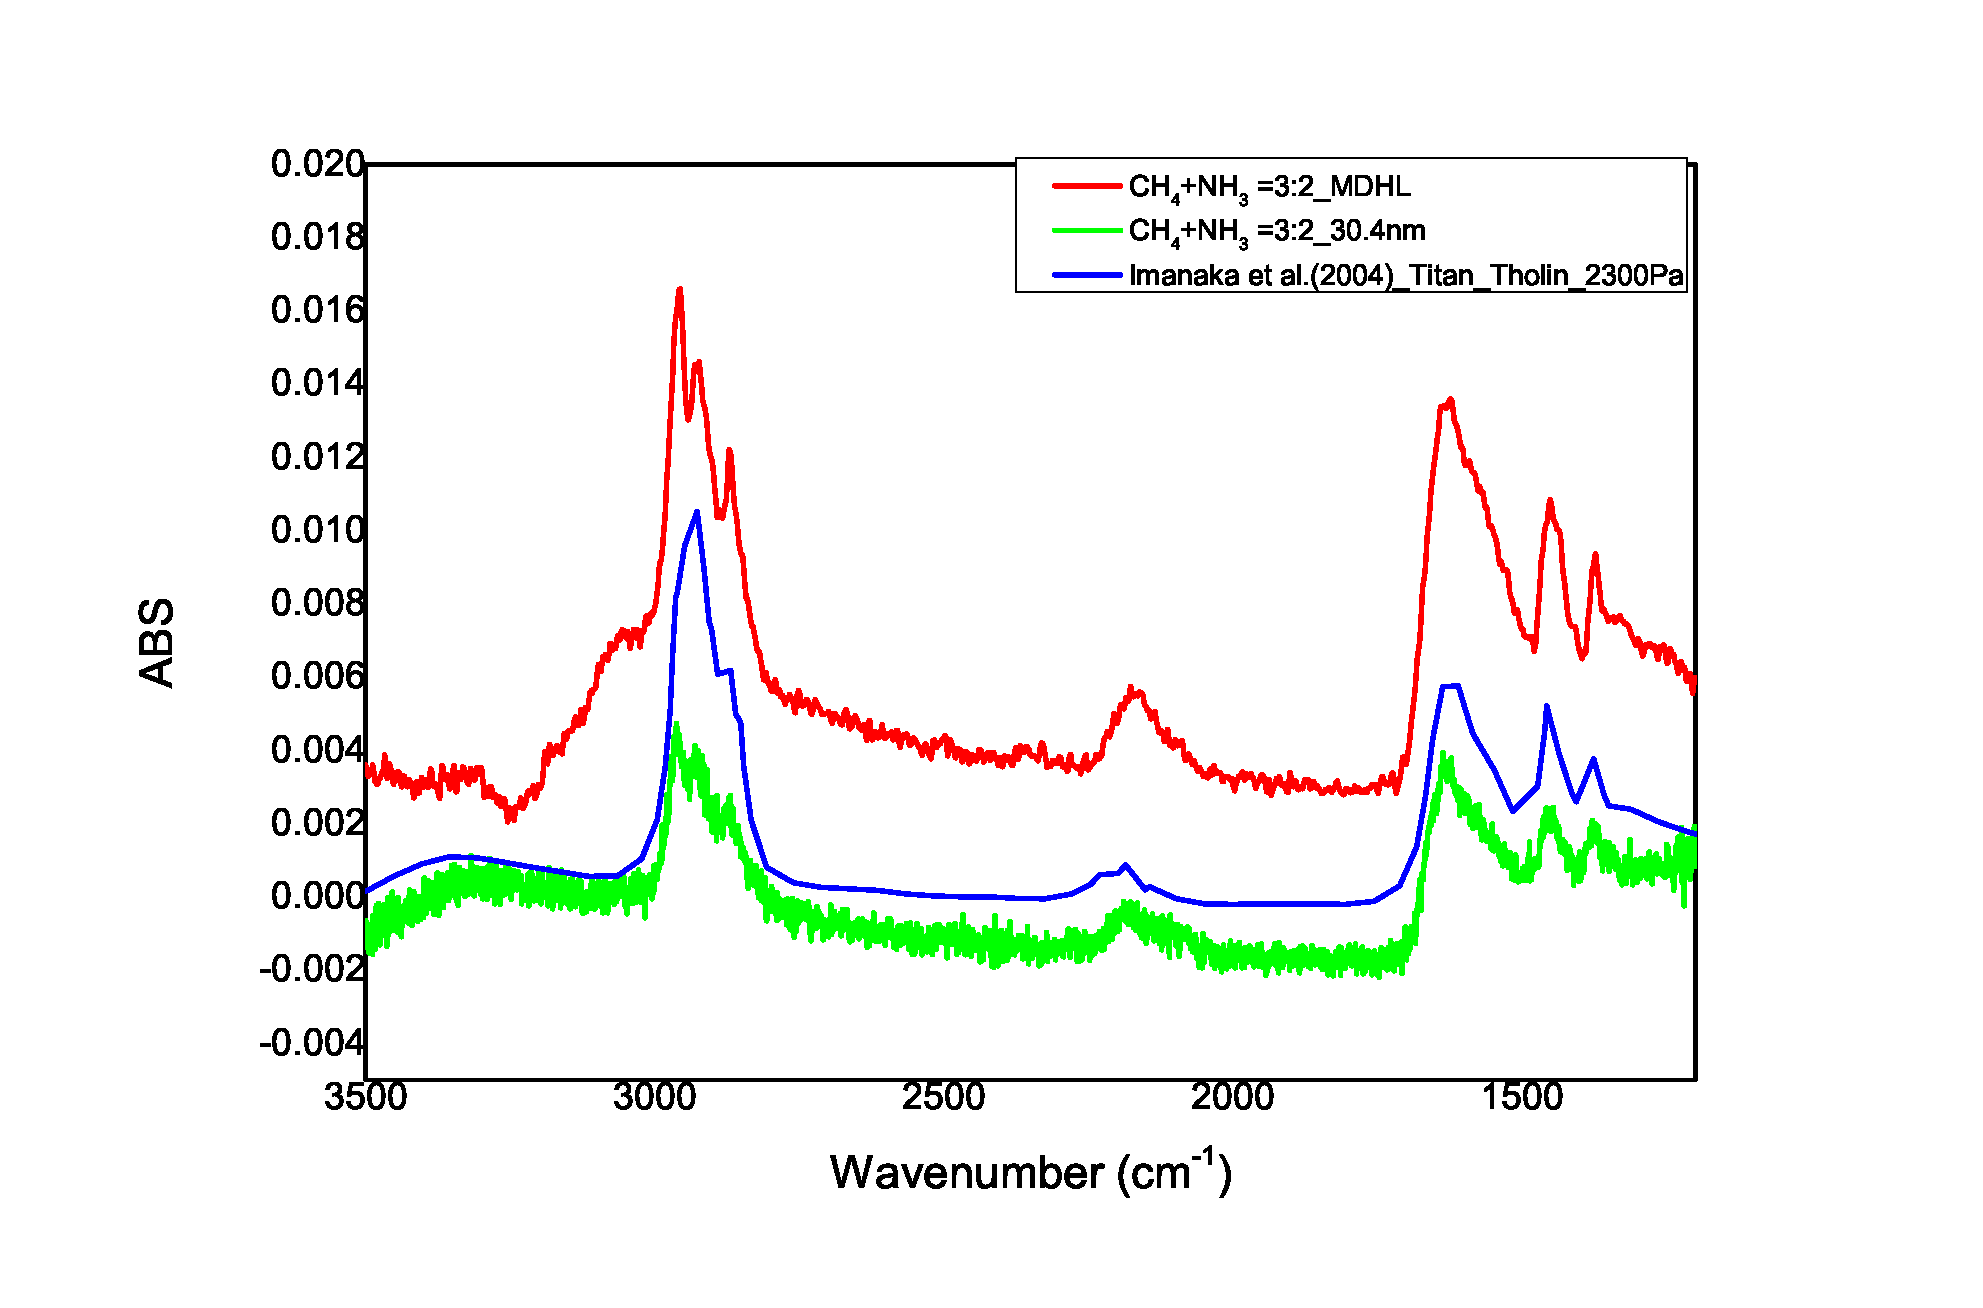
\includegraphics[width=\textwidth]{figures/chapter3/residue.eps}
\caption{The IR spectrum of residues in after CH$_4$+NH$_3$ = 3:2 experiments and the accumulate residues after MDHL experiments and NSRRC experiments.}
\label{fig:residues}
\end{figure}


\section{Conclusion} % should be in chapter 4?

The main product of VUV and EUV irradiated CH$_4$+NH$_3$ ice mixtures are C$_2$H$_6$ and CN$^-$. C$_3$H$_8$ is also produced by C$_2$H$_6$ or C$_2$H$_2$. We do several investigations towards CH$_4$+NH$_3$ ice mixtures. First, by changing ratio of CH$_4$ to NH$_3$ ice mixtures, CN$^-$ production is more effective in NH$_3$ dominated ice mixtures. While in contrast, C$_2$H$_6$ is the main product when CH$_4$ dominates. Second, by changing the photon source to EUV irradiation, the yield of C$_3$H$_8$ increases. The effective formation of C$_3$H$_8$ is not produced by C$_2$H$_6$ but by C$_2$H$_2$ and CH$_4$ because the ratio of C$_3$H$_8$ : C$_2$H$_6$ increases. This suggests that the CH$_2$ or CH fragmentation from CH$_4$ increases when photon energy increases. By studying the production efficiencies, the difference in photo-production yield is mainly caused by the reduction in photo-destruction cross-section in the reactants. Thirdly, in comparison with electron irradiation experiments, electron irradiation has a smaller absorption cross-sections, the percentage of yield is also smaller than VUV irradiated ice mixtures with similar ice thicknesses. Finally, we compare our residues obtained with laboratory produced Taitan tholins, the similar infra-red spectrum shows a similar functional groups in residues. Our result implies that the tholin on Charon should be similar to that of Titan.


               % 第三章    (自行寫入)
                                 % \backmatter

\cleardoublepage                         % 保證奇數頁為章節起始
\phantomsection
\addcontentsline{toc}{chapter}{索引}     % 將索引加入目錄中

\printindex

\cleardoublepage                         % 保證奇數頁為章節起始
\phantomsection
\addcontentsline{toc}{chapter}{參考文獻}     % 將參考文獻加入目錄中

\bibliographystyle{unsrt}      
%\bibliography{myfoo}                   % 或標準資料庫用法          
\begin{thebibliography}{20}          % 文獻少寫法
\bibitem{knu84}
Donald E. Knuth. \emph{{The TEXbook, Volume A of Computers and Typesetting}}. \hskip 1em plus 0.5em minus
 0.4em\relax Addison-Wesley, Reading, Massachusetts, second edition, 1984, ISBN 0-201-13448-9.\\
\url{http://www-cs-staff.stanford.edu/~knuth/index.html}

\bibitem{lam94}
Leslie Lamport. \emph{{\LaTeX{}: A Document Preparation System}}. \hskip 1em plus 0.5em minus 0.4em\relax Addison-Wesley, Reading, Massachusetts, second edition, 1994, ISBN 0-201-52983-1.

\bibitem{lo12a}
J.~LO, \emph{{eThinking in Circuits with PSpice}}.\hskip 1em plus
 0.5em minus 0.4em\relax Cavesbooks, Inc., 2012, \\ ISBN 978-957-41-8721-8.

\bibitem{lo12b}
------, \emph{{aThinking in Control with Matlab}}.\hskip 1em plus
0.5em minus 0.4em\relax Cavesbooks, Inc., 2012, \\ ISBN pending.

\bibitem{lo12c}
------, \emph{\LaTeX\ \& U 自助出版}.\hskip 1em plus
0.5em minus 0.4em\relax 中央敦煌, 北科文具部, 2012, \\ ISBN 978-957-41-9448-3.

\bibitem{lo12d}
------, \emph{Packages author of ncuthesis(CJK, Xe), bizcard, cnwritingCJK}.\hskip 1em plus
0.5em minus 0.4em\relax Free packages, 2012.\\
\url{https://code.google.com/p/ncu-thesis-latex-template/}
\bibitem{}
\emph{{Writing a thesis in \LaTeX}}
\url{http://texblog.org/}

\bibitem{126570}
Chinese character \textbackslash cjk within \textbackslash section\{\} does not work using pdflatex, + \textbackslash includegraphics, \hskip 1em plus
0.5em minus 0.4em\relax\\
\url{http://tex.stackexchange.com/a/126570}

\bibitem{79776}
\emph{Page numbers only appear on pages where a chapter starts}, \hskip 1em plus
0.5em minus 0.4em\relax\\
\url{http://tex.stackexchange.com/a/79776}
\end{thebibliography}                      % 少文獻寫法

                  % 文獻      (自行寫入)
%\stepcounter{chapter} % This is trick to keep the bookmark correct

\begin{appendA}

\fvset{frame=none,numbers=left,numbersep=3pt,firstline=1,lastline=300}
\VerbatimInput{ncuthesisXe.cls}
\todo[inline]{Xe與CJK是不同的.cls檔案,故這裏(appendi.tex)要改。}
\index{ncuthesis 環境!appendA}\index{\LaTeX!\textbackslash VerbatimInput}
\end{appendA}


\begin{appendB}

附錄資料於此載入,未設任何格式。
若性質不同可寫在不同附錄,即{\tt A}或{\tt B}。因只設計成兩
個附錄。若超過則需至{\tt ncuthesisXe(CJK)}複製後再改為{\tt C,D},...。每個附錄亦可有節({\tt section}),但沒有設計小節了({\tt subsection});方程式亦有不同於本文的編號,例如附錄二第一節的第一個方程式的編號如下。


\section{第一節}
有一個方程式(\ref{test})在第\pageref{test}頁
\begin{equation}
x+y=z  \label{test}
\end{equation}

\begin{equation}
1+1=2 
\end{equation}


\section{第二節}
猜猜看 第三個方程式的編號?\footnote{Ans: B.3,如何寫出編號?}
\[
r+s=t  \nonumber
\]
 \index{\LaTeX!\textbackslash pageref}
\renewcommand\thethm{B.\arabic{thm}}  
\index{\LaTeX!\textbackslash renewcommand}
\begin{thm}[附錄中之定理]
因為$\cdots\cdots$所以$\cdots\cdots$。
\end{thm}

其實小節、定理、引理、例題等皆依然可用在附錄裏 (但很少啦),只要加入這些指令於附錄前面,就可產生獨立於正文外之編號系統。

\begin{verbatim}
\renewcommand\thesubsection{B-\arabic{subsection}}  
\renewcommand\thethm{B.\arabic{thm}}  
\renewcommand\thelem{B.\arabic{lem}}  
\renewcommand\theex{B.\arabic{ex}} 
\end{verbatim}

如果在附錄A,該如何修改上述指令?
\vfil
\newpage
\section{自動化} \index{自動化}
此中央大學套件是依據中央大學論文規範而設計的,其他大專院校則有各自的規範,只要重新設計不同部分則各校亦可有自己的\LaTeX 格式檔;現將舉兩三例,讓有興趣的讀者發展屬於自己學校的套件格式且保留原始檔的完整性。
\index{ncuthesis 環境!onecol}

此法所有(多數)輸入參數可直接帶入,人工輸入只需一次。故稱自動化,例如
\begin{Verbatim}[frame=single,firstline=1,lastline=30,rulecolor=\color{red},label=Homework title page]
----- What follows go to the preamble
\makeatletter
\newcommand{\homework}{  % 定義開始
\newpage\partindent=0pt
{\centering
\sffamily\bfseries{\@dept}\\
\sffamily\bfseries{\@title}\\
\today\\}
\textit{\@author\hfill 班級 \hfill 學號}
\rule{\linewidth}{0.5mm}
}                        % 定義結束
\makeatother
\dept{工學院~機械系}
\title{自動控制 I, 2013 上/下學期}
\author{羅吉昌}
------ What follows go after \begin{document}
\homework  
此例是作業抬頭,讓想以\LaTeX 寫作業
的學生可以此套件寫作業;例如 第5章作業可這樣寫。
\setcounter{chapter}{5}  % 設定章數
\begin{pr}
此題的作業題目在此或不抄題 直接做答。
{\bf Solution:}
$\cdots$
\end{pr}
\end{Verbatim}       
其輸出如下兩頁所示。
為何不是下一頁而是下兩頁呢?因為封面,摘要,謝誌,甚至每一章的第一頁都應當在奇數頁出現 --- 面向上的一頁。 酷! 如何達成呢?記得\verb|\cleardoublepage|指令吧。就是它,記住了。
\cleardoublepage\phantomsection
\addcontentsline{toc}{subsection}{作業封面 }
\makeatletter
\newcommand{\homework}{%
\newpage                              
\setlength{\parindent}{0pt}  
{\centering
\sffamily\bfseries{\@dept}\\  
\sffamily\bfseries{\@title}\\
\today\\}
\textit{\@author\hfill 班級\hfill 學號}\footnote{因班級、學號無設計儲存變數,是新輸入,故直接寫入。} 
\rule{\linewidth}{0.5mm} 
}
\makeatother
\dept{工學院~機械系}
\title{自動控制 I, 2013 上/下學期}
\author{羅吉昌}
\homework
\index{\LaTeX!\textbackslash maketitle}
\index{ncuthesis 指令!\textbackslash homework}
\index{\LaTeX!\textbackslash linewidth}\index{\LaTeX!\textbackslash hfill}
\index{\LaTeX!\textbackslash sffamily} \index{\LaTeX!\textbackslash bfseries}
\index{\LaTeX!\textbackslash partindent}\index{\LaTeX!\textbackslash setlength}

此例是作業抬頭,例如 第5章作業可這樣寫。

\verb|\setcounter{chapter}{5}  % 設定章數|
\setcounter{chapter}{5}
\begin{pr}
此題的作業題目在此 或不抄題 直接做答。

{\bf Solution:}
$\cdots$
\end{pr}
%\setcounter{chapter}{2}
\index{\LaTeX!\textbackslash makeatletter}\index{\LaTeX!\textbackslash makeatother}\index{\LaTeX!\textbackslash renewcommand}

\rule{\linewidth}{0.5mm} 

這新的(非單獨)封面是定義\verb|\homework|的內容\footnote{若用{\tt titlepage}環境會產生單獨一頁。},只有簡單抬頭({\tt title})在頁眉,這樣就不需進入{\tt ncuthesisXe(CJK).cls}
檔改中央大學的結構,保持原始檔的完整性。
這簡單的抬頭({\tt title})設計是\LaTeX 非常重要的改寫計巧,因為它是標記{\tt markup}語言。此例題說明讀者可以上述概念重新以\verb|\renewcommand{\maketitle}|修改指令\verb|\maketitle|的內容,設計自己學校的論文封面\footnote{製作時將學校封面資訊拷貝至{\tt \textbackslash maketitle}修改,加入\LaTeX指令,主要是調整間距啦,一點都不難。書名頁亦同}。\par


再舉一自動化例題,這例題是改寫中英文摘要。

\begin{Verbatim}[frame=single,firstline=1,lastline=50,rulecolor=\color{red},label=New abstract]
----- What follows go to the preamble
\makeatletter
\renewenvironment{onecol}[1]  % 定義開始
{\cleardoublepage\phantomsection
\addcontentsline{toc}{subsection}{#1} % Or chapter
\begin{alwayssingle}
\thispagestyle{plain}
\begin{center}
{\Huge \bfseries #1}               % Or \Large and \large
\end{center}
\setlength{\parindent}{0pt}
{\Large 論文名稱:\@title \hfill頁數:101 頁
\par \vspace*{1ex}}
{\Large 校所系別:\@dept \par \vspace*{1ex}}
{\Large 畢業日期:\@degreedate \hfill 學位:碩/博士 
\par \vspace*{1ex}}
{\Large 研究生:\@author \hfill指導教授:
\par \vspace*{2ex}}
}
{\null \vfill
\end{alwayssingle}}           % 定義結束
\makeatother
------- What follows go to abstractcn.tex
\begin{abstractcn}{中文摘要}
關鍵字: 碩博士論文,體裁檔,\LaTeX,\XeLaTeX
\vspace{2ex}

\quad
這是新的中文摘要,與中大不同處是改寫{\tt onecol}環境的內容
,讓論文資訊在兩側而非置中結構,這樣就不需進入
{\tt ncuthesisXe(CJK).cls}檔
改中央大學的結構,保持原始檔的完整性。
\end{abstractcn}
\end{Verbatim}      
\index{\LaTeX!\textbackslash renewenvironment}
\index{\LaTeX!\textbackslash makeatletter}\index{\LaTeX!\textbackslash makeatother}




\makeatletter
\renewenvironment{onecol}[1]
{\cleardoublepage\phantomsection
\addcontentsline{toc}{subsection}{#1} % Or chapter
\begin{alwayssingle}
\thispagestyle{plain}
\begin{center}
{\Huge \bfseries #1}
\end{center}
\setlength{\parindent}{0pt}
{\Large 論文名稱:\@title \hfill頁數:101 頁
\par \vspace*{1ex}}
{\Large 校所系別:\@dept \par \vspace*{1ex}}
{\Large 畢業日期:\@degreedate \hfill 學位:\@degree \par \vspace*{1ex}}
{\Large 研究生:\@author \hfill指導教授:\@mprof \par \vspace*{2ex}}
}
{\null \vfill
\end{alwayssingle}}
\makeatother

\index{ncuthesis 指令!\textbackslash title}
\index{ncuthesis 指令!\textbackslash dept}
\index{ncuthesis 指令!\textbackslash degreedate}
\index{ncuthesis 指令!\textbackslash author}
\index{ncuthesis 指令!\textbackslash mprof}
\begin{abstractcn}
關鍵字: 碩博士論文,體裁檔,\LaTeX,\XeLaTeX
\vspace{2ex}

\quad

這是新的中文摘要,與中大不同處是改寫{\tt onecol}環境的內容,讓論文資訊在兩側而非置中結構,這樣就不需進入{\tt ncuthesisXe(CJK).cls}檔改中央大學的結構,保持原始檔的完整性。\index{論文資訊}。英文摘要亦同。

\begin{enumerate}
\item 頁數需自行填入,{\tt PDF} 閱讀器有顯示總頁數。
\item 所有論文相關資訊會自動帶入\footnote{{\tt titlepage}環境則無此功能。屬新輸入需自行填入,例如頁數。}。
\item 因前一例題設計作業抬頭時改寫了,故論文名稱是最新的。
\item 自動化\verb|\maketitle, \homework|指令\footnote{這兩指令都是做封面設計,名稱是設計者自訂,若相同則是要改寫現存指令,需用{\tt {\color{red}re}newcommand}改寫,若不同則是新指令需用{\tt newcommand}定義。}。及{\tt onecol}環境摘要是否可以用人工化的{\tt titlepage}環境產生?請看人工化一節說明。
\end{enumerate}
\end{abstractcn}
\index{ncuthesis 環境!abstractcn}\index{ncuthesis 環境!abstracten}

\begin{abstracten}        % 新英文摘要
Keywords: Redesign, Abstract
\vspace{2ex}

\quad  \index{\LaTeX!\textbackslash quad}

This is a renewed English abstract design (different from NCU). Again, for English abstract, just write your contents into the corresponding file (abstracten.tex.) All those headers will show on the top automatically.

\quad 
So, you have it. All the basis I can think of up to now, to help you generate a \LaTeX\ thesis file of your own.

\quad Last but not the least, hope you find this package valuable and would recommend it to others. 
\end{abstracten}


\section{手動化} \index{手動化}
自動化需要變數觀念
\begin{verbatim}
\<input>:使用者變數(user variables)。
\@<input>:內部變數(internal variables)。
後者只可以在 \makeatletter ... \makeatother 環境內處理。
\end{verbatim}
手動化則只需{\tt titlepage}環境。下一例是拷貝上一節自動化的例題,將變數設定改為人工輸入:簡言之,自動化$\Rightarrow$手動化。

用\verb|\begin{titlepage} ... \end{titlepage}|以自行填入方式製作,不設\verb|\author, \dept, \mprof|等輸入變數,完全手動({\tt Free style, manually}),故彈性最大,但重複的資訊需自行多次輸入,故較費工,適合個人化採用。若每個人都用相同介面則採變數設計較佳。
\begin{Verbatim}[frame=single,firstline=1,lastline=40,rulecolor=\color{red},label=Self-made title page]
----- What follows go after \begin{document} command
\begin{titlepage}
\setcounter{page}{67}
\begin{center}
有些學校\\
這裏有些\\
其他資訊\\
\vspace{1.5cm}
{\Huge\bfseries 學校名稱 \\[2cm]}
{\Large\bfseries 系所名稱 \\[1cm]}
{\Large\bfseries 論文題目(中) \\子標題\\ [1cm]} 
{\Large\bfseries 論文題目(英) \\子標題 \\ [2cm]}
A Thesis\\
Submitted to Department of $\ldots$\\
in Partial Fulfillment of the Requirements\\
for the Degree of Master/Doctor\\
in \\
\vspace*{1cm}
\begin{minipage}{0.45\textwidth}
\begin{flushleft}
研究生: $\ldots$
\end{flushleft}
\end{minipage}
\begin{minipage}{0.45\textwidth}
\begin{flushright}
指導教授:$\ldots$ \\
共同指導:$\ldots$
\end{flushright}
\end{minipage}\\
\vspace*{1.5cm}

\includegraphics[scale=0.5]{NCUlogo.jpg}
\par
中~華~民~國~一百零二~年~七~月
\end{center}
\end{titlepage}
\end{Verbatim}

其結果如下兩頁所示。為何不是下一頁而是下兩頁呢?因為封面,摘要,謝誌,甚至每一章的第一頁都應當在奇數頁出現 --- 面向上的一頁。 酷! 如何達成呢?記得\verb|\cleardoublepage|指令吧。就是它,記住了。

\cleardoublepage\phantomsection
\addcontentsline{toc}{subsection}{自製封面} 
\begin{titlepage}
\thispagestyle{plain}
\setcounter{page}{67}
\begin{center}
有些學校\\
這裏有些\\
其他資訊\\
\vspace{1.5cm}
{\Huge\bfseries 學校名稱 \\[2cm]}
{\Large\bfseries 系所名稱 \\[1cm]}
{\Large\bfseries 論文題目(中) \\子標題\\ [1cm]} 
{\Large\bfseries 論文題目(英) \\子標題 \\ [2cm]}
A Thesis\\
Submitted to Department of $\ldots$\\
in Partial Fulfillment of the Requirements\\
for the Degree of Master/Doctor\\
in \\
\vspace*{1cm}
\begin{minipage}{0.45\textwidth}
\begin{flushleft}
研究生: $\ldots$
\end{flushleft}
\end{minipage}
\begin{minipage}{0.45\textwidth}
\begin{flushright}
指導教授:$\ldots$ \\
共同指導:$\ldots$
\end{flushright}
\end{minipage}\\
\vspace*{1.5cm}

\includegraphics[scale=0.5]{NCUlogo.jpg}
\par
中~華~民~國~一百零二~年~七~月
\end{center}
\end{titlepage}

再舉一中文摘要例題。

\begin{Verbatim}[frame=single,firstline=1,lastline=30,rulecolor=\color{red},label=Another abstract]
----- What follows go after \begin{document}
\cleardoublepage\phantomsection
\addcontentsline{toc}{subsection}{又一摘要} % Or chapter
\begin{titlepage}
\thispagestyle{plain}
\setcounter{page}{69}                    % 自設頁碼
\begin{center}
{\Huge \bfseries 又一摘要}
\end{center}
\setlength{\parindent}{0pt}
{\Large 論文名稱:$\ldots$ \hfill頁數:101 頁
\par \vspace*{1ex}}
{\Large 校所系別:$\ldots$ \par \vspace*{1ex}}
{\Large 畢業日期:$\ldots$ \hfill 學位:碩/博士 
\par \vspace*{1ex}}
{\Large 研究生:  $\ldots$ \hfill指導教授:$\ldots$ 
\par \vspace*{2ex}}

\vspace{1cm}

關鍵字:自動化,手動化
\vspace{2ex}

這是用人工化{\tt titlepage}環境寫的新中文摘要,
英文摘要亦同。

\end{titlepage}
\end{Verbatim}

可產生

\cleardoublepage\phantomsection
\addcontentsline{toc}{subsection}{又一摘要}  % section can be changed to chapter
\begin{titlepage}
\thispagestyle{plain}
\setcounter{page}{69}                                % 自設頁碼
\begin{center}
{\Huge \bfseries 又一摘要}
\end{center}
\setlength{\parindent}{0pt}
{\Large 論文名稱:$\ldots$ \hfill頁數:101 頁
\todo[inline]{別忘了完稿時,頁碼要自己填入正確數字。}
\par \vspace*{1ex}}
{\Large 校所系別:$\ldots$ \par \vspace*{1ex}}
{\Large 畢業日期:$\ldots$ \hfill 學位:碩/博士 \par \vspace*{1ex}}
{\Large 研究生:    $\ldots$ \hfill指導教授:$\ldots$ \par \vspace*{2ex}}

\vspace{1cm}

關鍵字:自動化,手動化
\vspace{2ex}

這是用手動{\tt titlepage}環境寫的新中文摘要,英文摘要亦同。

\begin{itemize}
\item $\ldots$ 表示要自己手動填入,不是用變數法自動帶入。
\item 手動化{\tt titlepage}環境永遠設頁碼為1,但摘要常常不是第一頁,故需以\verb|\setcounter{page}{69}|設頁碼。
\item 如何將此手動化改為自動化?逆向回去\footnote{將 {\tt titlepage}的內容以{\tt \textbackslash newenvironment}定義{\tt abstractcn}環境,然後將人工輸入變數{\tt \textbackslash<input>}以{\tt \textbackslash \char64<input>取代。最後以{\tt \textbackslash makeatletter ... \textbackslash makeatother}包住。}}。還是不懂!!!再研究自動化第二題,有無了解此兩題互為"\,反函數":自動化$\Leftarrow$手動化,它們之間的差異是什麼?
\item 以人工化{\tt titlepage}環境修改此套件為個人使用的封面、中英文摘要,謝誌,其實相對而言很簡單。自動化則需了解變數的用法。
\item 所以學到技巧了嗎?同樣的觀念亦可用來設計其他大專院校封面、中、英文摘要、謝誌等因與中央大學論文格式不同而需重新設計又希望保持原始檔的完整性。
\end{itemize}
\end{titlepage}

%\section{投影片}
\clearpage\phantomsection
\addcontentsline{toc}{section}{投影片} 

\includepdf[pages=-,scale=0.9]{beamertest.pdf} 
\end{appendB}               % 若有需要 使用appendA/B環境
 

\clearpage
\end{CJK}                        
%---------------------
\clearpage
\bookbone                        % 短書脊製作
{\centering\layout}
\end{document}                   % 本文結束
